
\section*{CHƯƠNG 4. TRIỂN KHAI VÀ KIỂM THỬ}
\setcounter{section}{4}
\setcounter{subsection}{0} %LƯU Ý MỖI LẦN THÊM CHƯƠNG MỚI CẦN THÊM CÂU NÀY ĐỂ RESET THỨ TỰ CỦA SUBSECTON VỀ 1
\setcounter{table}{0} % LƯU Ý SAU MỖI LẦN GỌI BẢNG HAY HÌNH ẢNH PHẢI THÊM CÂU NÀY ĐỂ RESET THỨ TỰ
\setcounter{figure}{0} %% LƯU Ý SAU MỖI LẦN GỌI BẢNG HAY HÌNH ẢNH PHẢI THÊM CÂU NÀY ĐỂ RESET THỨ TỰ
\addcontentsline{toc}{section}{\numberline{}CHƯƠNG 4. TRIỂN KHAI VÀ KIỂM THỬ}

\subsection{Công nghệ sử dụng}

\subsubsection{Thiết kế giao diện website}

\paragraph{ReactJs}
\mbox{}

ReactJs là framework được chúng em sử dụng để lập trình giao diện website, dưới đây là phần giới thiệu về ReactJs cũng
như những tính năng sẽ được chúng em sử dụng trong ứng dụng này.

ReactJs là một framework mã nguồn mở phát triển bởi Facebook, được sử dụng để xây dựng giao diện website nhanh chóng. 
ReactJs sử dụng ngôn ngữ lập trình JavaScript, là một ngôn ngữ hiện đại và linh hoạt, giúp tạo ra các giao diện đẹp mắt và hiệu ứng mượt mà trên môi trường internet browser.
\begin{figure}[H]
  \centering
  
\includegraphics[width=12cm,height=5.4cm]{Images/reactjs_cover.png}
  \caption[Logo ReactJs]{\bfseries \fontsize{12pt}{0pt}
  \selectfont Logo ReactJs}
  \label{reactjs_cover} %đặt tên cho ảnh
\end{figure}

Một số điểm nổi bật của ReactJs được chúng em sử dụng bao gồm:


\begin{itemize}
  \item Giao diện được xây dựng dễ dàng với tư duy Component, có thể tuỳ biến tái sử dụng những component giống nhau để code ngắn gọn dễ hiểu hơn
  \item Tích hợp nhanh chóng: ReactJs hỗ trợ việc code và render giao diện một cách nhanh chóng tối ưu hoá được thời gian phát triển giao diện
  \item Tương thích đa nền tảng: ReactJs tương thích với hầu hết các internet browser hiện nay như: chrome, firefox, coc coc, microsoft edge, opera, brave,...
\end{itemize}

\subsubsection{Server}
\paragraph{Javascript}
\mbox{}

JavaScript là một ngôn ngữ lập trình thông dịch, đa mục đích và được sử dụng phổ biến trên web. Nó ra đời vào năm 1995 bởi Brendan Eich, khi còn là một ngôn ngữ lập trình đơn giản để cung cấp tính năng tương tác và hiệu ứng động cho trang web \cite{js_1}. Tuy nhiên, từ đó đến nay, JavaScript đã trở thành một trong những ngôn ngữ lập trình quan trọng nhất trên thế giới, vượt qua giới hạn trang web và mở rộng sang nhiều lĩnh vực phát triển phần mềm khác nhau.
JavaScript là một ngôn ngữ lập trình linh hoạt, mạnh mẽ và phổ biến, có nhiều ưu điểm vượt trội như tích hợp tốt với trình duyệt, đa dạng kiểu dữ liệu, khả năng thực hiện bất đồng bộ, và cộng đồng phát triển mạnh mẽ. JavaScript đã định hình lại cách các ứng dụng web tương tác và được sử dụng rộng rãi trong nhiều lĩnh vực phát triển phần mềm. Sự phát triển của các framework và thư viện JavaScript giúp người phát triển xây dựng các ứng dụng web phức tạp và mạnh mẽ một cách dễ dàng và hiệu quả hơn.




\paragraph{NodeJs}
\mbox{}

Node.js là một nền tảng phát triển ứng dụng mã nguồn mở cực kỳ mạnh mẽ và đa dạng, giúp các nhà phát triển xây dựng các ứng dụng web và dịch vụ server-side với hiệu suất cao và khả năng mở rộng linh hoạt \cite{nodejs_1}. Được ra đời vào năm 2009, Node.js đã nhanh chóng trở thành một trong những công nghệ phổ biến nhất trong cộng đồng lập trình viên và được ứng dụng rộng rãi trong các dự án phức tạp cũng như các ứng dụng thời gian thực. 

\begin{figure}[H]
  \centering
  \includegraphics[width=16cm,height=8cm]{Images/server/tech_used/nodejs_arch.jpg}
  \caption[Kiến trúc của NodeJS]{\bfseries \fontsize{12pt}{0pt}
  \selectfont Kiến trúc của NodeJS}
  \label{ble_services} %đặt tên cho ảnh
\end{figure}
Trong quá trình triển khai ứng dụng, Node.js hỗ trợ dễ dàng tích hợp với các công cụ triển khai (deployment tools) như Docker và Kubernetes, giúp đơn giản hóa quá trình triển khai và vận hành ứng dụng trên các môi trường khác nhau.

Tổng kết lại, Node.js là một nền tảng phát triển ứng dụng đa dạng và mạnh mẽ, với nhiều ưu điểm nổi trội như kiến trúc không đồng bộ, tích hợp với JavaScript, đa nền tảng, hỗ trợ ứng dụng thời gian thực, và cộng đồng lớn hỗ trợ phong phú. Với những lợi ích đáng kể này, Node.js đã trở thành một lựa chọn ưu việt cho việc xây dựng các ứng dụng web và dịch vụ server-side hiệu quả và mạnh mẽ.

\paragraph{MySQL}
\mbox{}

MySQL là một hệ quản trị cơ sở dữ liệu mã nguồn mở phổ biến và mạnh mẽ, được sử dụng rộng rãi trong nhiều ứng dụng và dự án phát triển phần mềm. MySQL ra đời vào năm 1995, do công ty TcX phát triển và sau đó được mua lại bởi công ty MySQL AB. Hiện nay, MySQL thuộc sở hữu của Oracle Corporation sau khi Oracle mua lại Sun Microsystems - công ty mẹ của MySQL AB vào năm 2010. \cite{mysql_1}

MySQL là hệ quản trị cơ sở dữ liệu (DBMS - Database Management System) dựa trên mô hình quan hệ (relational database) và sử dụng ngôn ngữ truy vấn cấu trúc (Structured Query Language - SQL) để thực hiện các thao tác truy vấn dữ liệu. Mô hình quan hệ của MySQL cho phép lưu trữ và quản lý dữ liệu trong các bảng có mối quan hệ với nhau, tạo điều kiện để thực hiện các truy vấn phức tạp và hiệu quả. \cite{myql_2}

Tóm lại, MySQL là một hệ quản trị cơ sở dữ liệu mã nguồn mở mạnh mẽ và phổ biến, được sử dụng rộng rãi trong nhiều ứng dụng và dự án phát triển phần mềm. Với tính năng hiệu suất cao, khả năng mở rộng linh hoạt, tính bảo mật và quản lý người dùng, sự hỗ trợ từ cộng đồng và tích hợp với nhiều công cụ phát triển, MySQL đã trở thành một lựa chọn ưu việt cho việc quản lý và xử lý cơ sở dữ liệu.

\paragraph{PostgreSQL}
\mbox{}

PostgreSQL là một hệ quản trị cơ sở dữ liệu quan hệ đối tượng (ORDBMS) mã nguồn mở, miễn phí, được phát triển bởi cộng đồng toàn cầu. PostgreSQL bắt nguồn từ dự án POSTGRES của Đại học California tại Berkeley vào những năm 1980. Nó chính thức được phát hành lần đầu tiên vào năm 1996 dưới tên PostgreSQL.

PostgreSQL hỗ trợ một loạt các kiểu dữ liệu đa dạng và phong phú, giúp nó trở nên linh hoạt và mạnh mẽ trong việc quản lý dữ liệu. Do đó trong hệ thống đề xuất chúng em đã sử dụng PostgreSql để lưu trữ dữ liệu tin nhắn, giúp cải thiện khả năng quản lý dữ liệu và tăng tốc độ truy vấn tin nhắn.
\paragraph{Postman}
\mbox{}

Postman là một ứng dụng máy tính được sử dụng phổ biến trong quá trình phát triển và kiểm thử các dịch vụ web (web service) và các API (Application Programming Interface) \cite{postman_1}. Được phát triển bởi công ty Postman Inc., ứng dụng này cung cấp một giao diện đơn giản và dễ sử dụng để gửi các yêu cầu HTTP (HTTP request) và nhận các phản hồi (response) từ các API. Postman giúp người phát triển dễ dàng thử nghiệm và kiểm tra tính năng, hiệu năng và bảo mật của các dịch vụ web và API, từ đó đảm bảo chất lượng và độ tin cậy của ứng dụng.

Postman đã trở thành một công cụ quan trọng và không thể thiếu trong quá trình phát triển và kiểm thử các ứng dụng và dịch vụ web. Sự dễ dàng sử dụng, tích hợp và tự động hóa giúp tăng cường năng suất và chất lượng của quá trình phát triển, đồng thời giảm thiểu nguy cơ lỗi và tối ưu hóa hiệu suất của ứng dụng.

\paragraph{Docker}
\mbox{}

Docker là một nền tảng mã nguồn mở được thiết kế để tự động hóa việc triển khai, mở rộng và quản lý các ứng dụng trong các container. Container là một đơn vị phần mềm nhẹ, có thể chạy độc lập và bao gồm tất cả các thành phần cần thiết để chạy ứng dụng, bao gồm mã nguồn, thư viện, và cấu hình hệ thống.

Docker được phát triển bởi Docker, Inc. và lần đầu tiên được ra mắt vào năm 2013. Từ đó, Docker đã nhanh chóng trở thành một công cụ quan trọng trong quá trình phát triển phần mềm, đặc biệt là trong các môi trường DevOps.

Docker không chỉ hỗ trợ các lập trình viên và các chuyên gia IT trong việc phát triển và triển khai ứng dụng, mà còn đóng vai trò quan trọng trong việc thúc đẩy các phương pháp làm việc hiện đại như Continuous Integration/Continuous Deployment (CI/CD) và microservices. Với Docker, các doanh nghiệp có thể đẩy nhanh quá trình phát triển phần mềm, cải thiện chất lượng sản phẩm, và giảm thiểu chi phí vận hành.

\begin{figure}[H]
  \centering
  
\includegraphics[scale=0.8]{Images/server/deploy/docker.png}
  \caption[Docker]{\bfseries \fontsize{12pt}{0pt}
  \selectfont Docker}
  \label{docker} %đặt tên cho ảnh
\end{figure}


\paragraph{GPT-4 API}
\mbox{}

GPT API (Generative Pre-trained Transformer API) 
là một dịch vụ được cung cấp bởi OpenAI cho phép các nhà phát triển tích hợp khả năng xử lý ngôn ngữ tự nhiên (NLP) vào ứng dụng, 
trang web hoặc dịch vụ của họ. 

\begin{figure}[H]
  \centering
  
\includegraphics[scale=0.9]{Images/server/ai/openai.png}
  \caption[OpenAi API]{\bfseries \fontsize{12pt}{0pt}
  \selectfont OpenAi API}
  \label{openai} %đặt tên cho ảnh
\end{figure}

\begin{enumerate}[a)]
\item Model GPT-4

GPT-4 là phiên bản mới nhất và tiên tiến nhất trong dòng mô hình GPT của OpenAI. 
Được xây dựng dựa trên nền tảng của các phiên bản trước, 
GPT-4 mang lại nhiều cải tiến đáng kể:

\begin{itemize}
  \item Khả năng hiểu biết tốt hơn: GPT-4 có khả năng hiểu ngữ cảnh và ngữ nghĩa tốt hơn, giúp tạo ra các phản hồi chính xác và phù hợp hơn.
  \item Tăng cường khả năng tạo văn bản: Với kho dữ liệu huấn luyện rộng lớn và đa dạng, GPT-4 có thể tạo ra văn bản tự nhiên và mạch lạc, thậm chí trong các ngữ cảnh phức tạp.
  \item Tích hợp đa nhiệm: GPT-4 API cho phép người dùng dễ dàng tuỳ biến và đào tạo dựa trên dữ liệu có sẵn của họ để tạo ra các trợ lý ảo phù hợp với đặc điểm của hệ thống
\end{itemize}

\item Ứng dụng của GPT-4 trong đồ án
\mbox{}

Vì những ưu điểm trên chúng em đã tích hợp GPT API vào việc xây dựng trợ lý ảo dùng để tư vấn cho người dùng về hệ thống, 
cách sử dụng thiết bị và cách tích hợp thiết bị của hệ thống, ngoài ra trợ lý ảo còn giúp người dùng tự động hoá việc sử dụng hệ thống.
\end{enumerate}

\subsection{Triển khai ứng dụng}
Trong quá trình triển khai ứng dụng, chúng em áp dụng quy trình phát triển ứng dụng CI/CD để phát triển và xây dựng hệ thống. Để triển khai hệ thống theo đúng quy trình CI/CD thì chúng em đã sử dụng các dịch vụ, VPS server để triển khai server API và website, Docker để tự động deploy ứng dụng, MySQL Server để quản lý cơ sở dữ liệu, Github để quản lý code.

\subsubsection{Quy trình CI/CD}
CI/CD là viết tắt của Continuous Integration (CI) và Continuous Delivery (CD). Có thể hiểu nó được kết hợp bởi quy trình Tích hợp liên tục và Phân phối liên tục. CI/CD giúp tạo ra sản phẩm cuối cùng nhanh chóng dựa trên kết hợp công việc của mỗi cá nhân.



\begin{figure}[H]
  \centering
  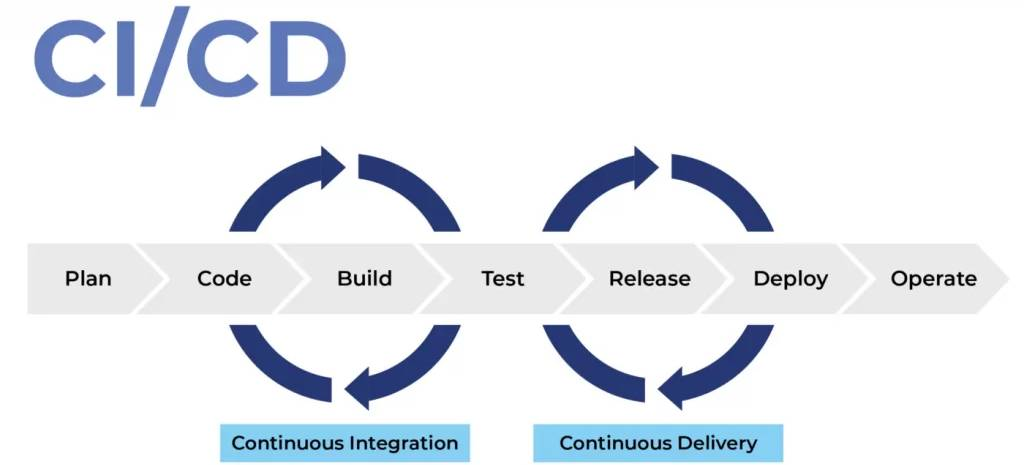
\includegraphics[scale=0.3]{Images/server/deploy/ci-cd.png}
  \caption[Quy trình CI/CD]{\bfseries \fontsize{12pt}{0pt}
  \selectfont Quy trình CI/CD}
  \label{ci-cd} %đặt tên cho ảnh
\end{figure}

Hệ thống được xây dựng theo quy trình CI/CD, sử dụng các công nghệ như docker, github, vps server để tự động hoá quy trình deploy hệ thống. Từ đó việc kiểm thử được diễn ra thường xuyên, dễ dàng và chính xác hơn. 

\subsubsection{Kiến trúc Microservices}

Kiến trúc Microservices là một phương pháp phát triển phần mềm trong đó một ứng dụng lớn được chia thành nhiều dịch vụ nhỏ độc lập với nhau. Mỗi dịch vụ thực hiện một chức năng cụ thể và giao tiếp với các dịch vụ khác qua các giao thức giao tiếp nhẹ như HTTP/HTTPS, JSON, WebHooks, Notification.

\begin{figure}[H]
  \centering
  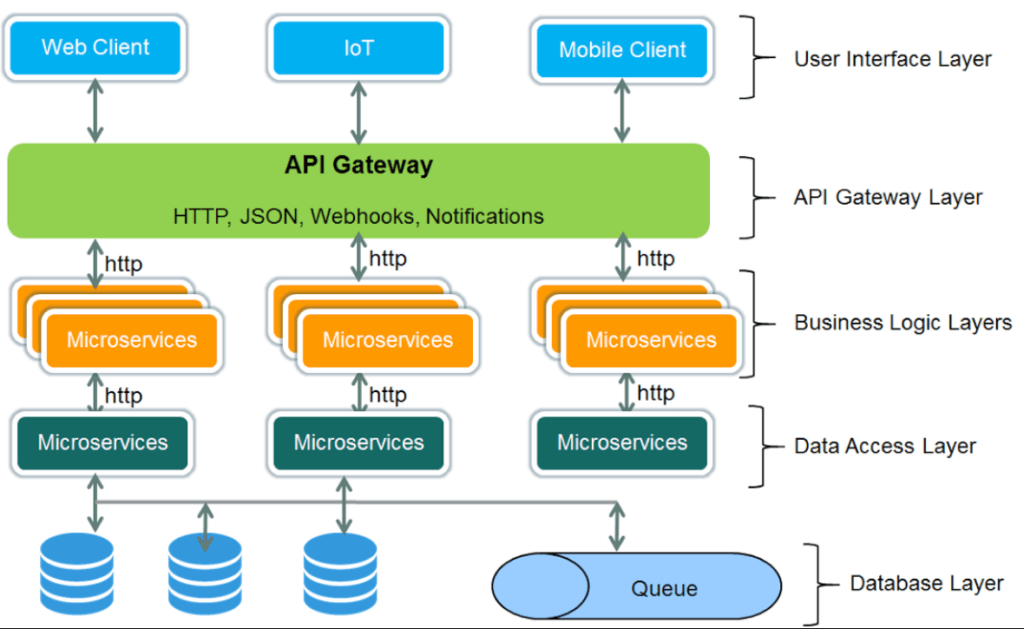
\includegraphics[scale=0.3]{Images/server/deploy/micro-service.png}
  \caption[Kiến trúc Microservices]{\bfseries \fontsize{12pt}{0pt}
  \selectfont Kiến trúc Microservices}
  \label{micro-service} %đặt tên cho ảnh
\end{figure}

Trong hệ thống chúng em đã tách riêng phần chat, server, mobile app và giao diện người dùng, phát triển từng phần thành các ứng dụng độc lập với nhau kết nối qua API. Điều này giúp việc code nhanh hơn, dữ liệu được lưu trữ phân tán dễ dàng bảo trì và nâng cấp 
\subsubsection{Triển khai Server và ứng dụng web trên máy chủ VPS}
  Cài đặt các dịch vụ cần thiết cho máy chủ VPS sử dụng hệ điều hành Unbutu như: nodejs, npm, pm2, nginx, docker, github,...

  \begin{figure}[H]
    \centering
    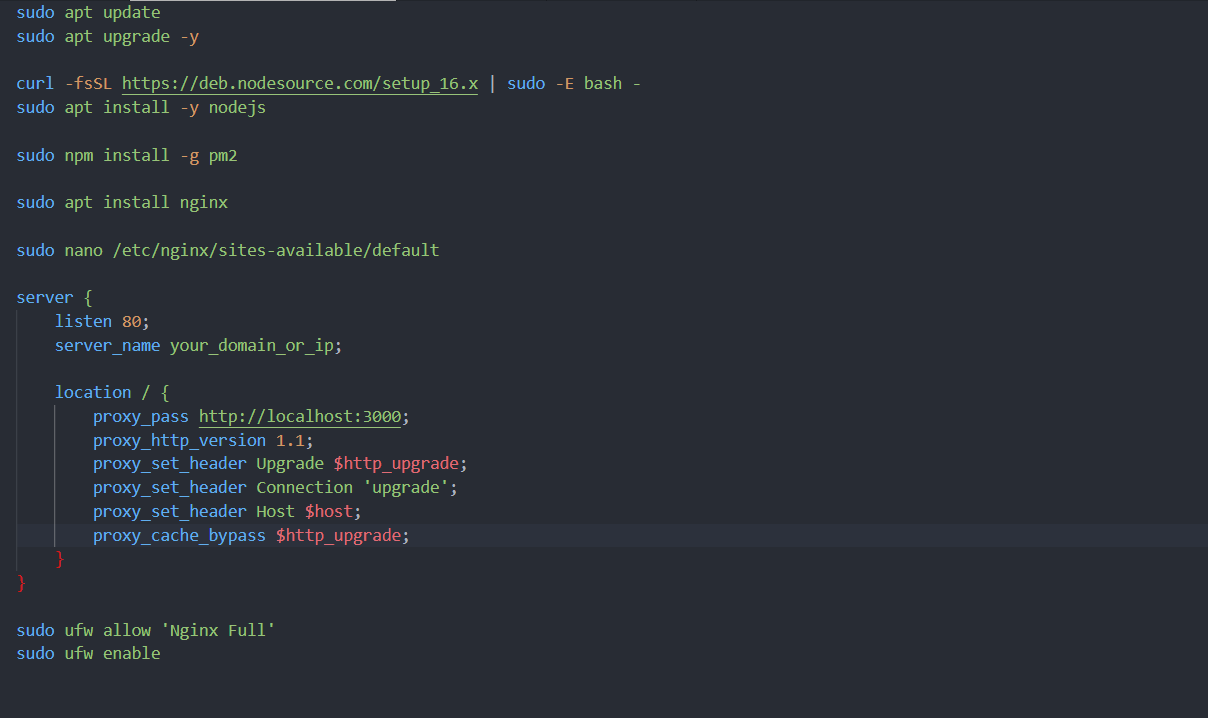
\includegraphics[scale=0.5]{Images/server/deploy/config_server.png}
    \caption[Cài đặt các dịch vụ cần thiết cho server]{\bfseries \fontsize{12pt}{0pt}
    \selectfont Cài đặt các dịch vụ cần thiết cho server}
    \label{create_server} %đặt tên cho ảnh
  \end{figure}

  Sau khi thành công chúng ta có thể kéo code về từ github và build ứng dụng bằng docker 
  
  \begin{figure}[H]
    \centering
    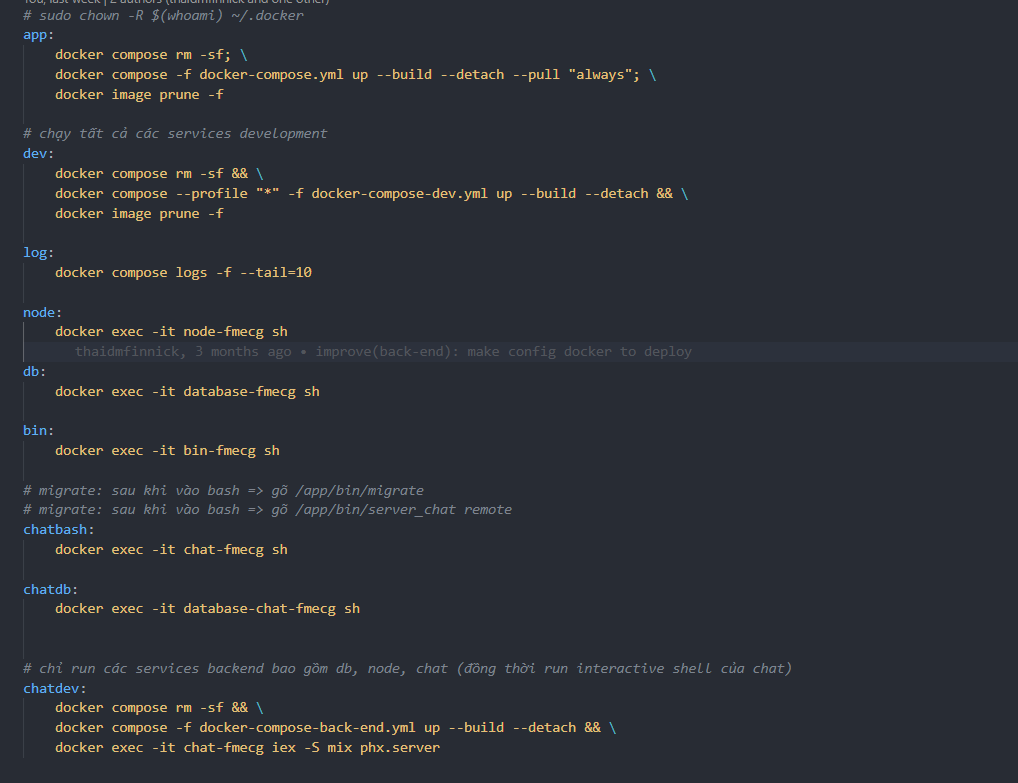
\includegraphics[scale=0.5]{Images/server/deploy/docker-run.png}
    \caption[Khởi chạy hệ thống bằng docker]{\bfseries \fontsize{12pt}{0pt}
    \selectfont Khởi chạy hệ thống bằng docker}
    \label{docker-run} %đặt tên cho ảnh
  \end{figure}

  Lúc này Docker sẽ tự động build và chạy tát cả các dịch vụ trong hệ thống như: server-ecd, server-chat, ui-web, mysql server, postgreSQL server. Sau khi chạy hoàn tất các cục ứng dụng sẽ được hiển thị lên như sau:

  \begin{figure}[H]
    \centering
    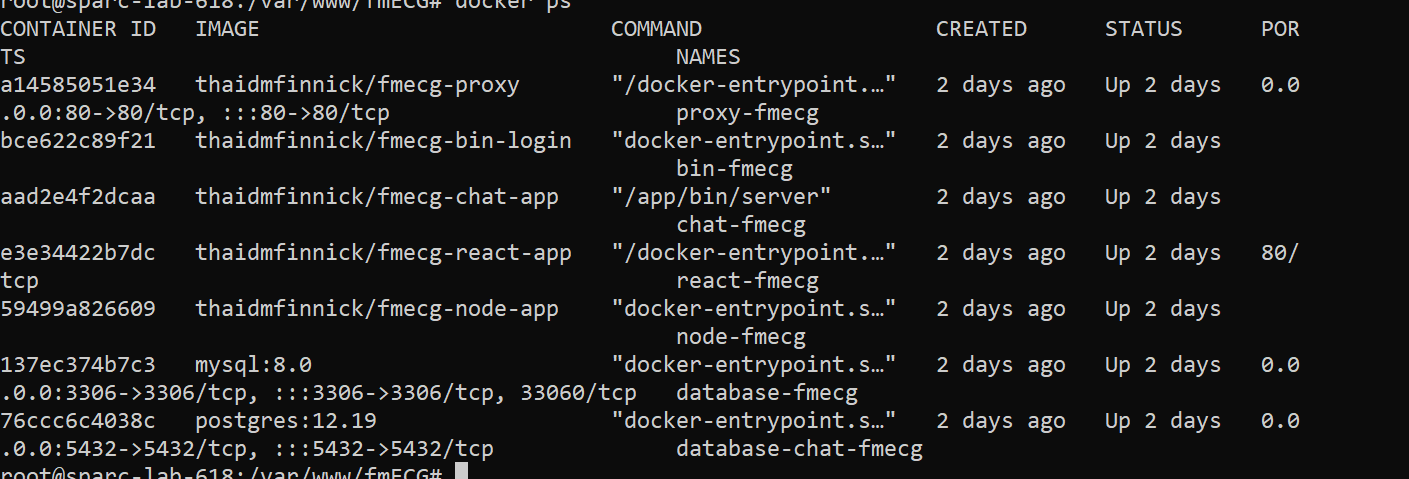
\includegraphics[scale=0.5]{Images/server/deploy/docker-container.png}
    \caption[Trạng thái hoạt động của các dịch vụ]{\bfseries \fontsize{12pt}{0pt}
    \selectfont Trạng thái hoạt động của các dịch vụ}
    \label{docker-container-status} %đặt tên cho ảnh
  \end{figure}

  Cài đặt Github Action workflow để tự động update code khi có code mới được ghép vào hệ thống 
 
  \begin{figure}[H]
    \centering
    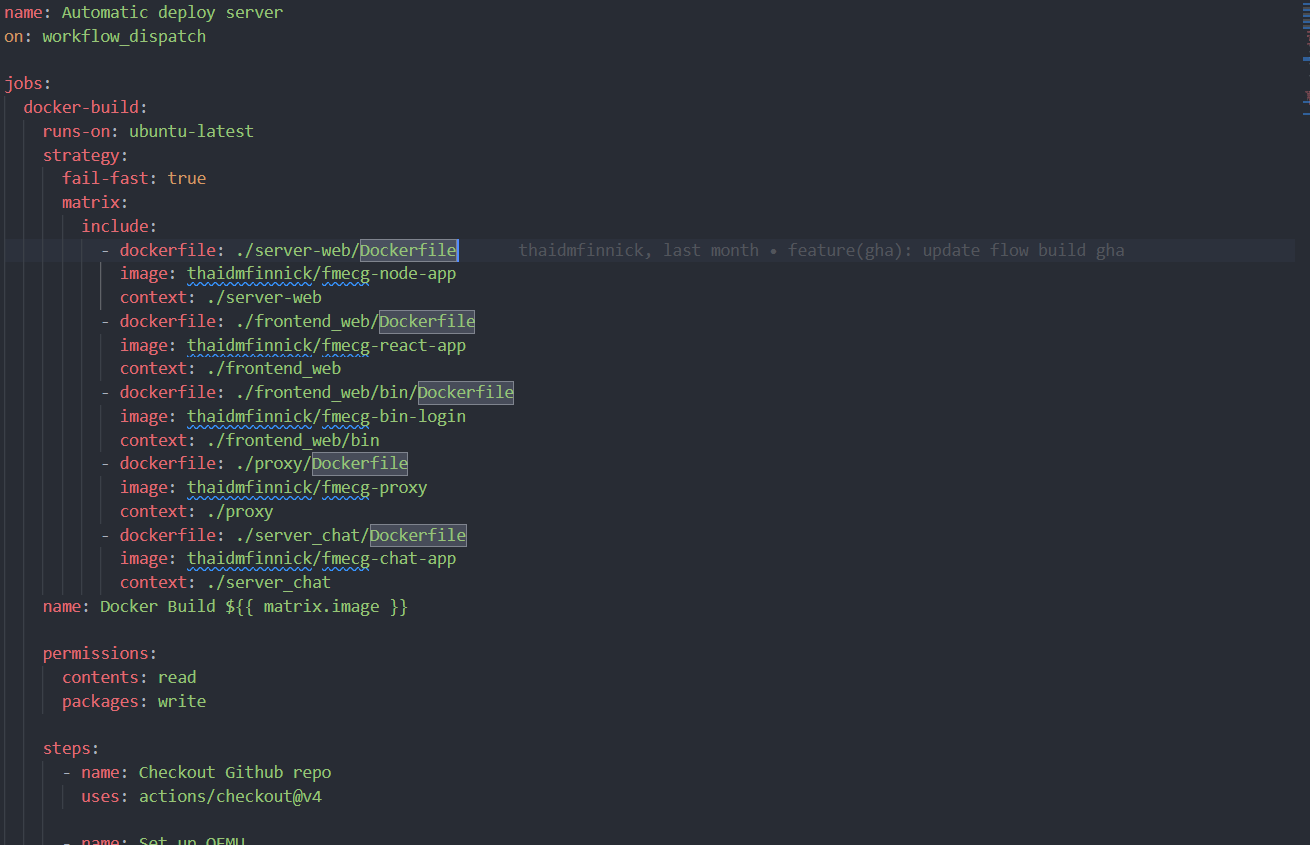
\includegraphics[scale=0.5]{Images/server/deploy/github-workflow.png}
    \caption[Cài đặt github-workflow]{\bfseries \fontsize{12pt}{0pt}
    \selectfont Cài đặt github-workflow}
    \label{github-workflow} %đặt tên cho ảnh
  \end{figure}

  Tạo API lắng nghe phản hồi từ github, khi có code mới github sẽ tự động gửi dữ liệu về api đã tạo.

  \begin{figure}[H]
    \centering
    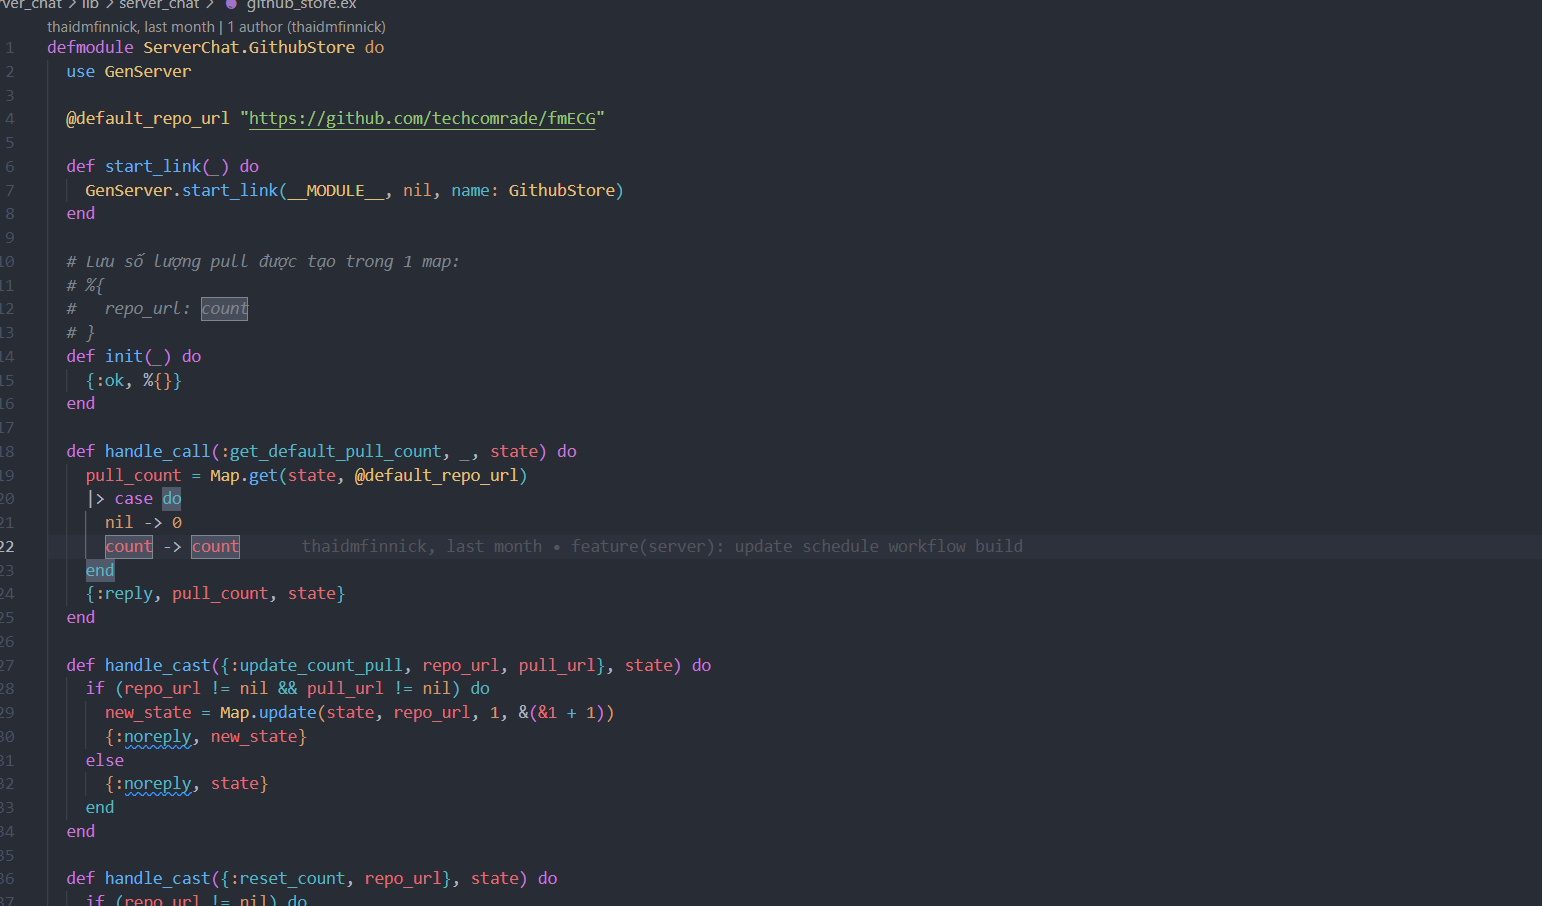
\includegraphics[scale=0.5]{Images/server/deploy/github-api.png}
    \caption[API nhận dữ liệu từ github]{\bfseries \fontsize{12pt}{0pt}
    \selectfont API nhận dữ liệu từ github}
    \label{github-api} %đặt tên cho ảnh
  \end{figure}

  Sau khi hoàn tất các bước hệ thống sẽ tự động build các cục dịch vụ trên github, và khi build xong code mới sẽ được gửi về VPS server để chạy
  \begin{figure}[H]
    \centering
    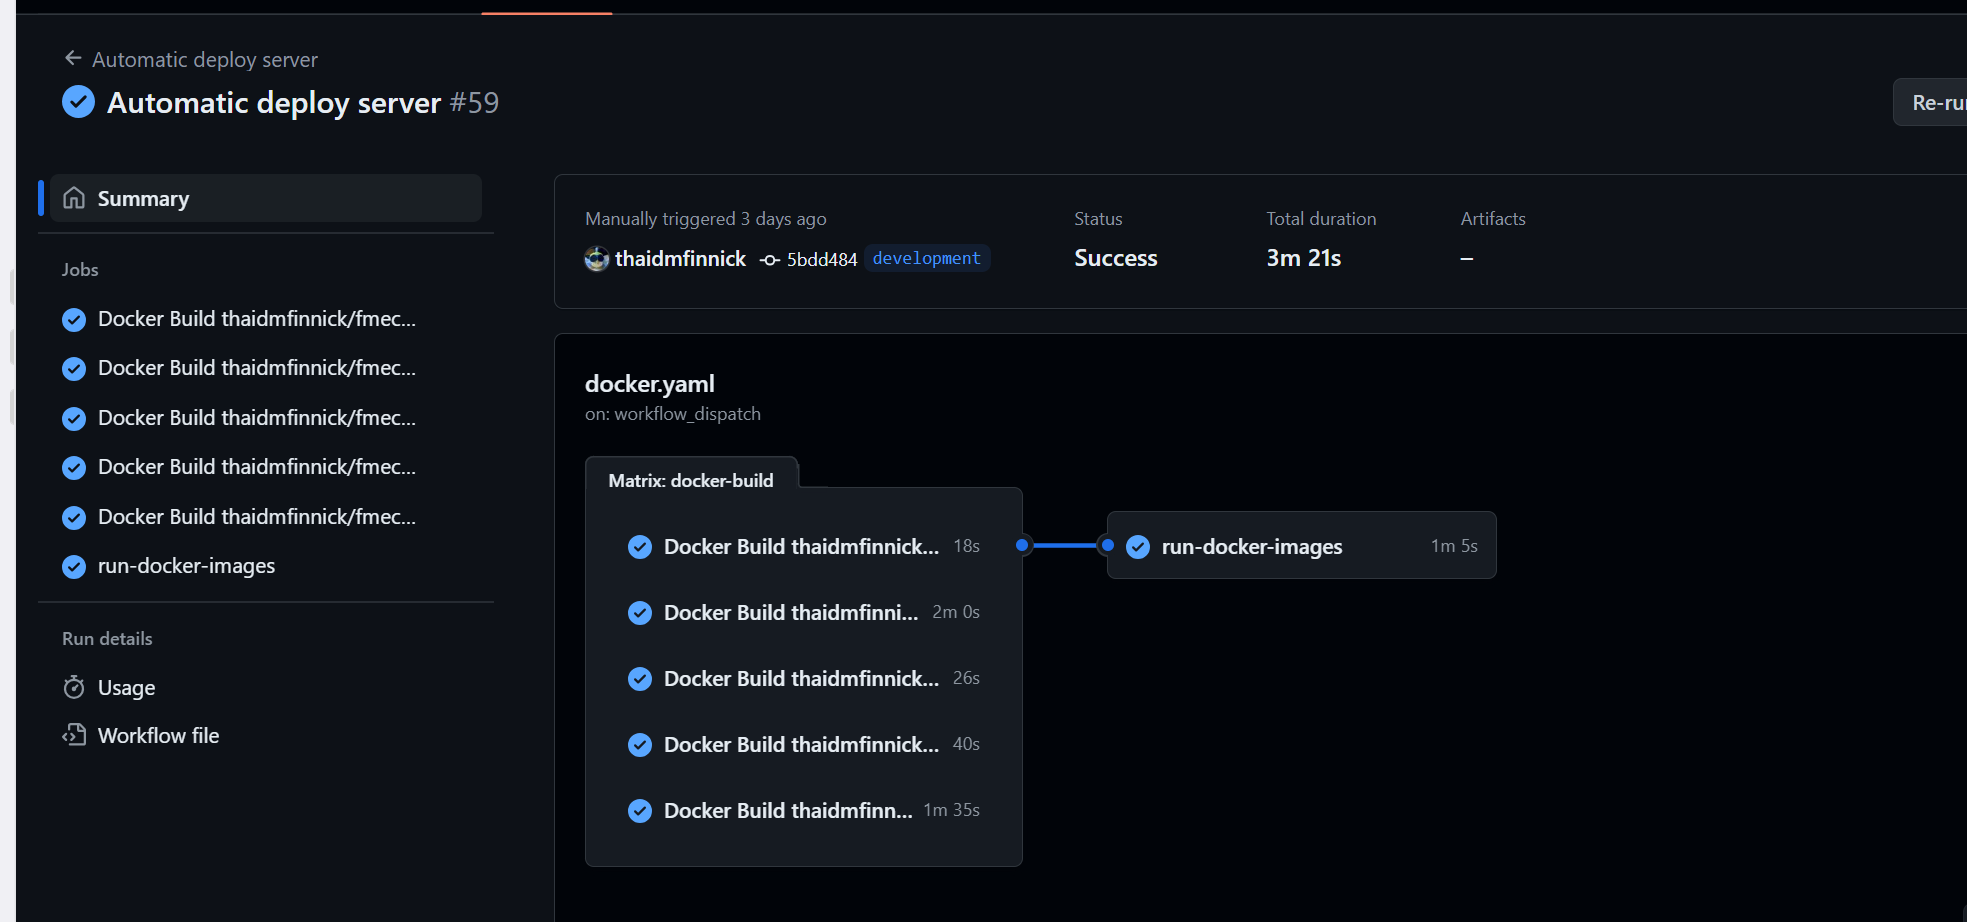
\includegraphics[scale=0.4]{Images/server/deploy/auto-deploy.png}
    \caption[Tự động build dữ liệu trên github]{\bfseries \fontsize{12pt}{0pt}
    \selectfont Tự động build dữ liệu trên github}
    \label{github-build} %đặt tên cho ảnh
  \end{figure}
  Hệ thống sẽ tự động quét vào 11 giờ 30 phút tối hàng ngày nếu có code mới được cập nhật sẽ tự động deploy lại phiên bản mới của hệ thống.
  Sau mỗi lượt deploy cập nhật các tính năng mới thì chúng em sẽ tiến hành kiểm thử chi tiết.
  Backup và giám sát cơ sở dữ liệu: Chúng em đã thiết lập các chính sách sao lưu định kỳ cho cơ sở dữ liệu và lưu các bản sao lưu lên trên github để đảm bảo an toàn cho dữ liệu và khả năng khôi phục trong trường hợp xảy ra sự cố.


\subsubsection{Tiến hành tạo model và huấn luyện AI}
Đầu tiên, tạo project trên OpenAI API để đăng ký model AI sử dụng cho hệ thống.
\begin{figure}[H]
  \centering
  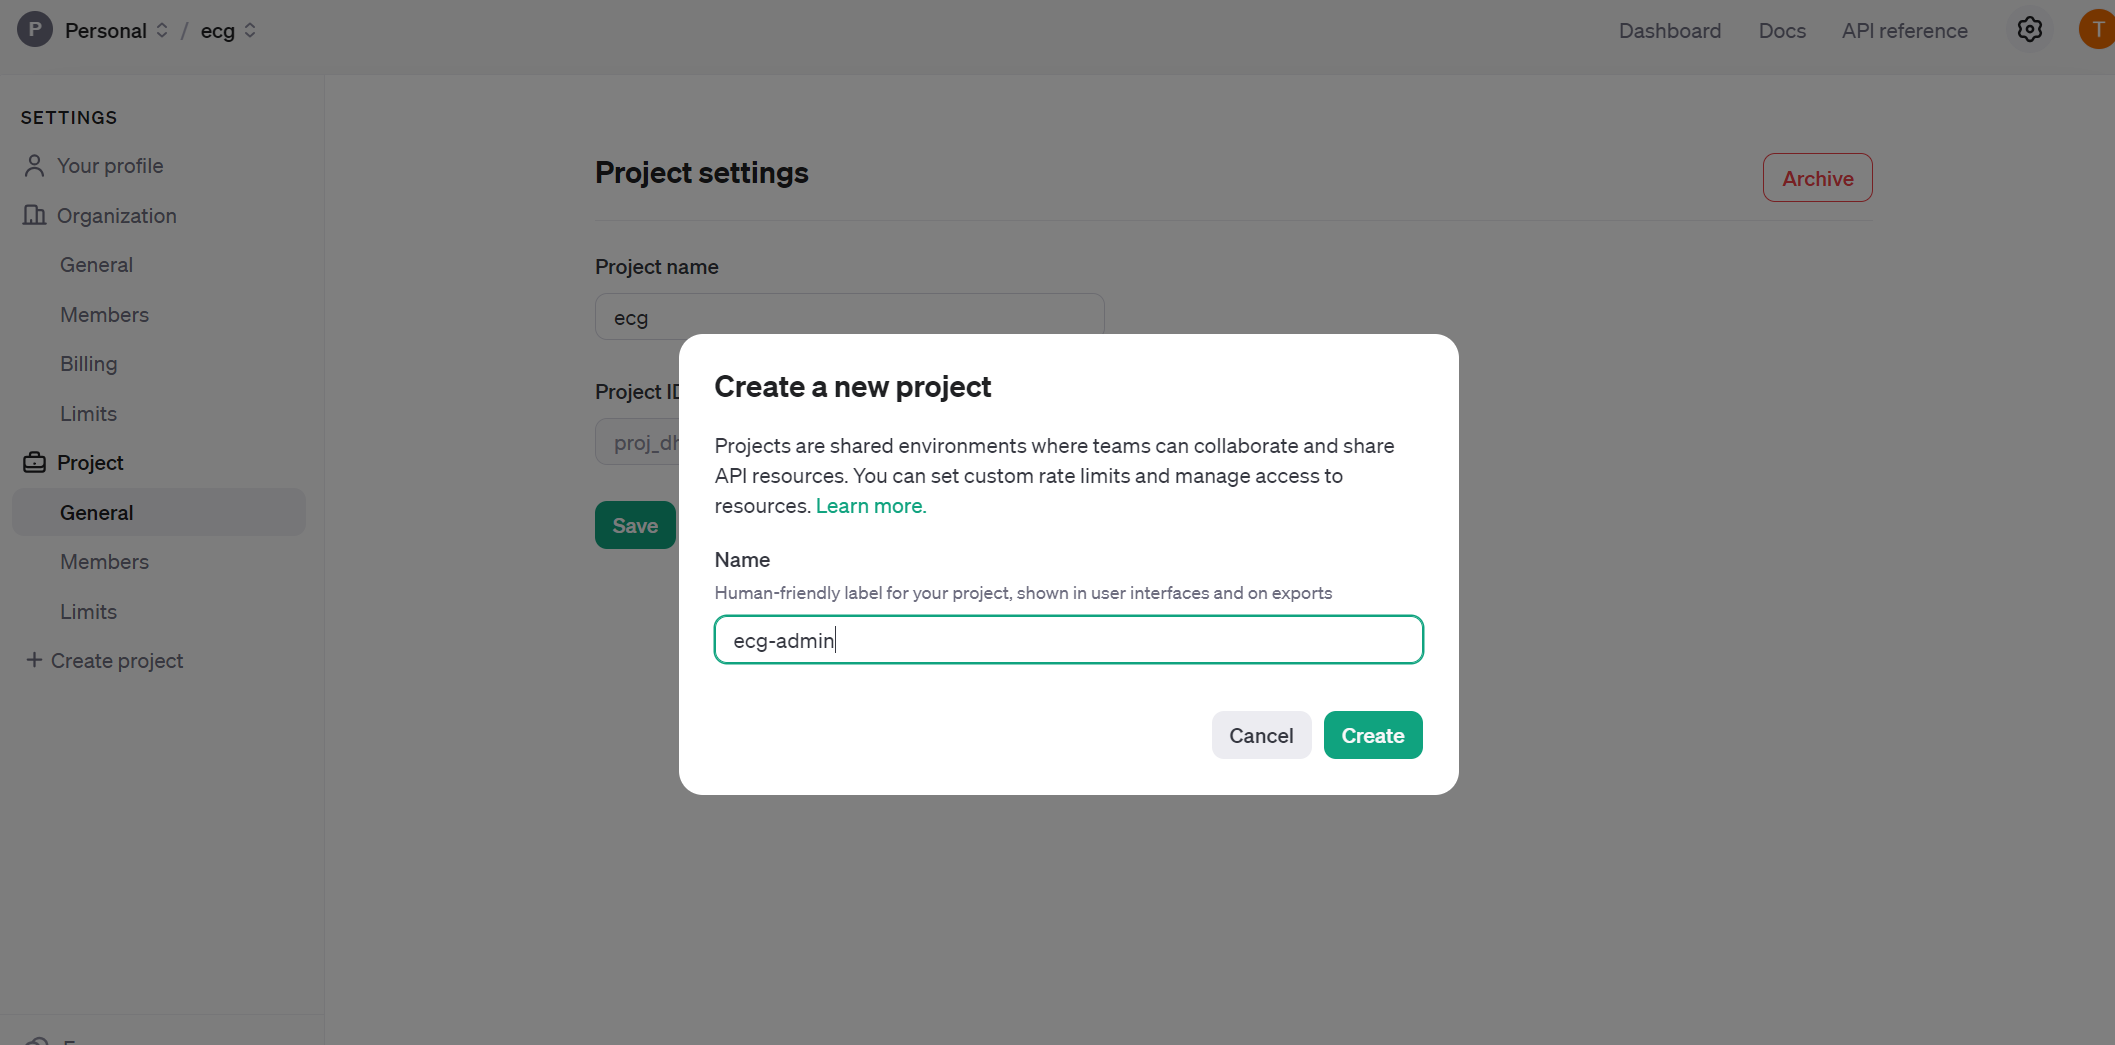
\includegraphics[scale=0.4]{Images/server/ai/create-project.png}
  \caption[Tạo project trên openai api]{\bfseries \fontsize{12pt}{0pt}
  \selectfont Tạo project trên openai api}
  \label{create-ai-project} %đặt tên cho ảnh
\end{figure}

Lựa chọn model AI hợp lý, ở đây chúng em chọn model GPT-4. Sau đó đưa ra hướng dẫn chung về cấu trúc, công việc của trợ lý ảo cần làm

\begin{figure}[H]
  \centering
  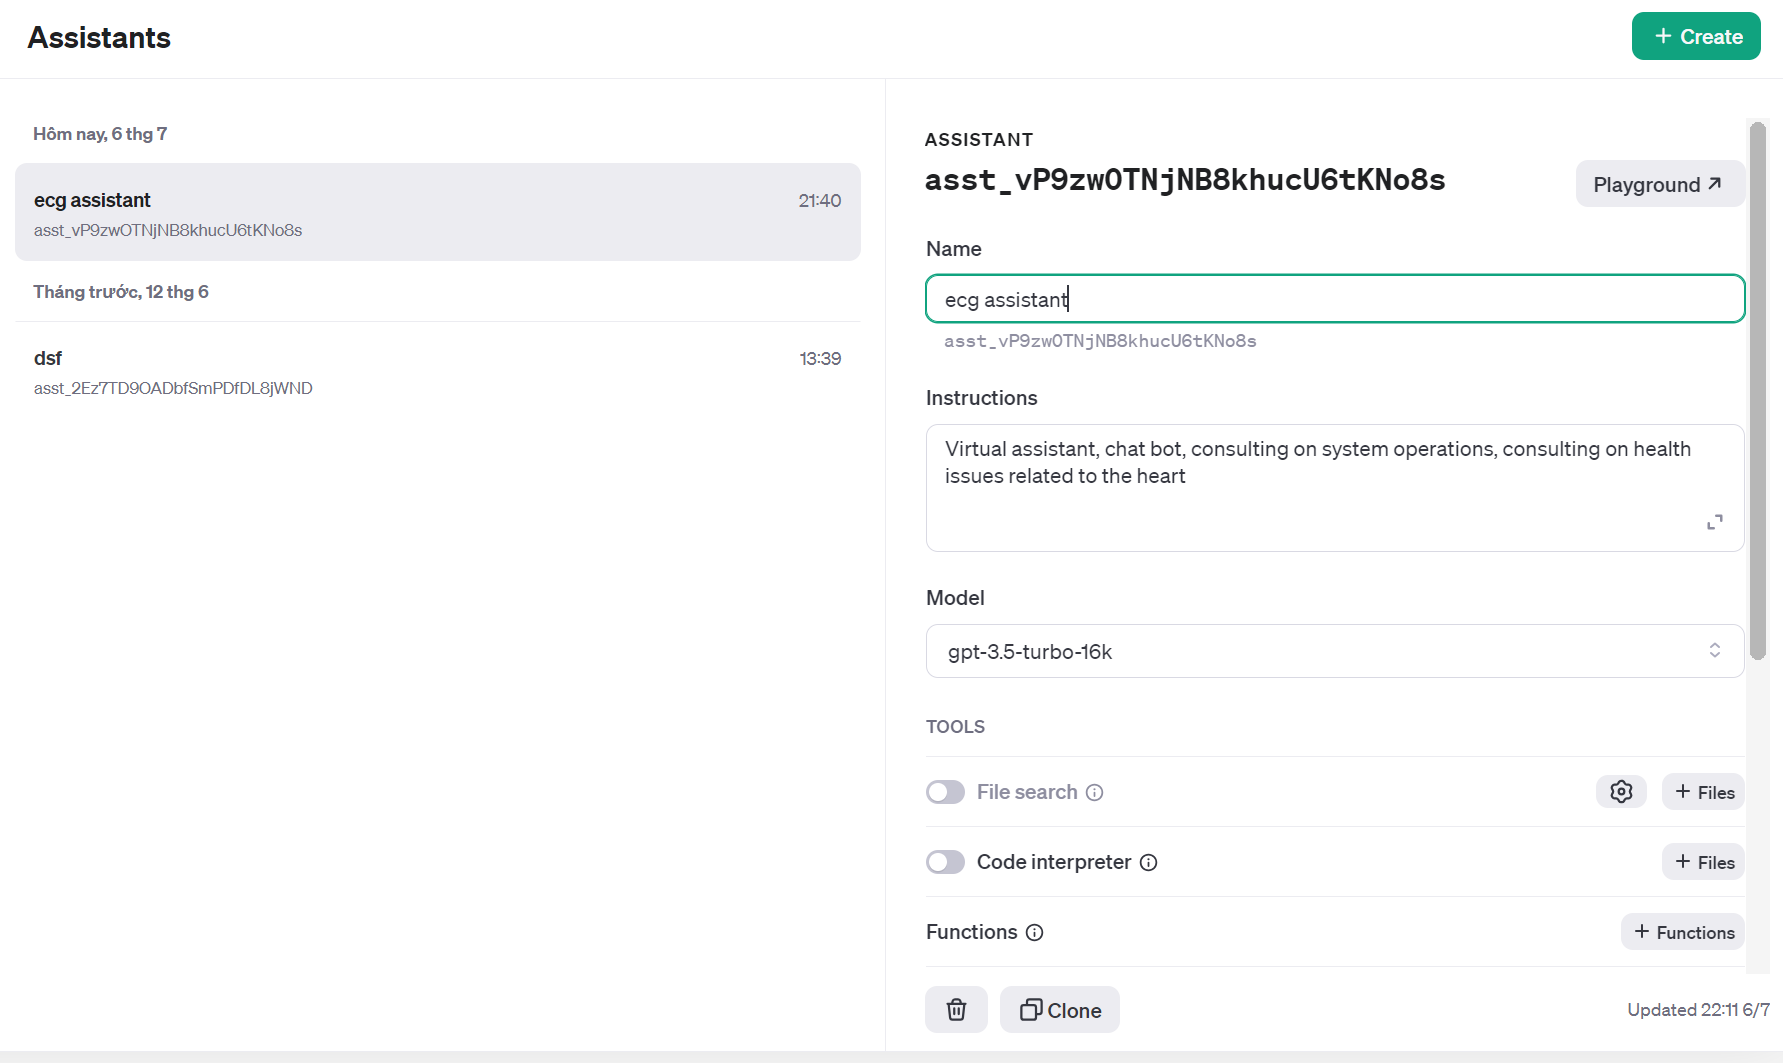
\includegraphics[scale=0.4]{Images/server/ai/create-assistant.png}
  \caption[Tạo model AI phù hợp]{\bfseries \fontsize{12pt}{0pt}
  \selectfont Tạo model AI phù hợp}
  \label{create-ai-assistant} %đặt tên cho ảnh
\end{figure}

Tạo khoá bảo mật để có thể liên kết trực tiếp với model GPT-4 thông qua API 

\begin{figure}[H]
  \centering
  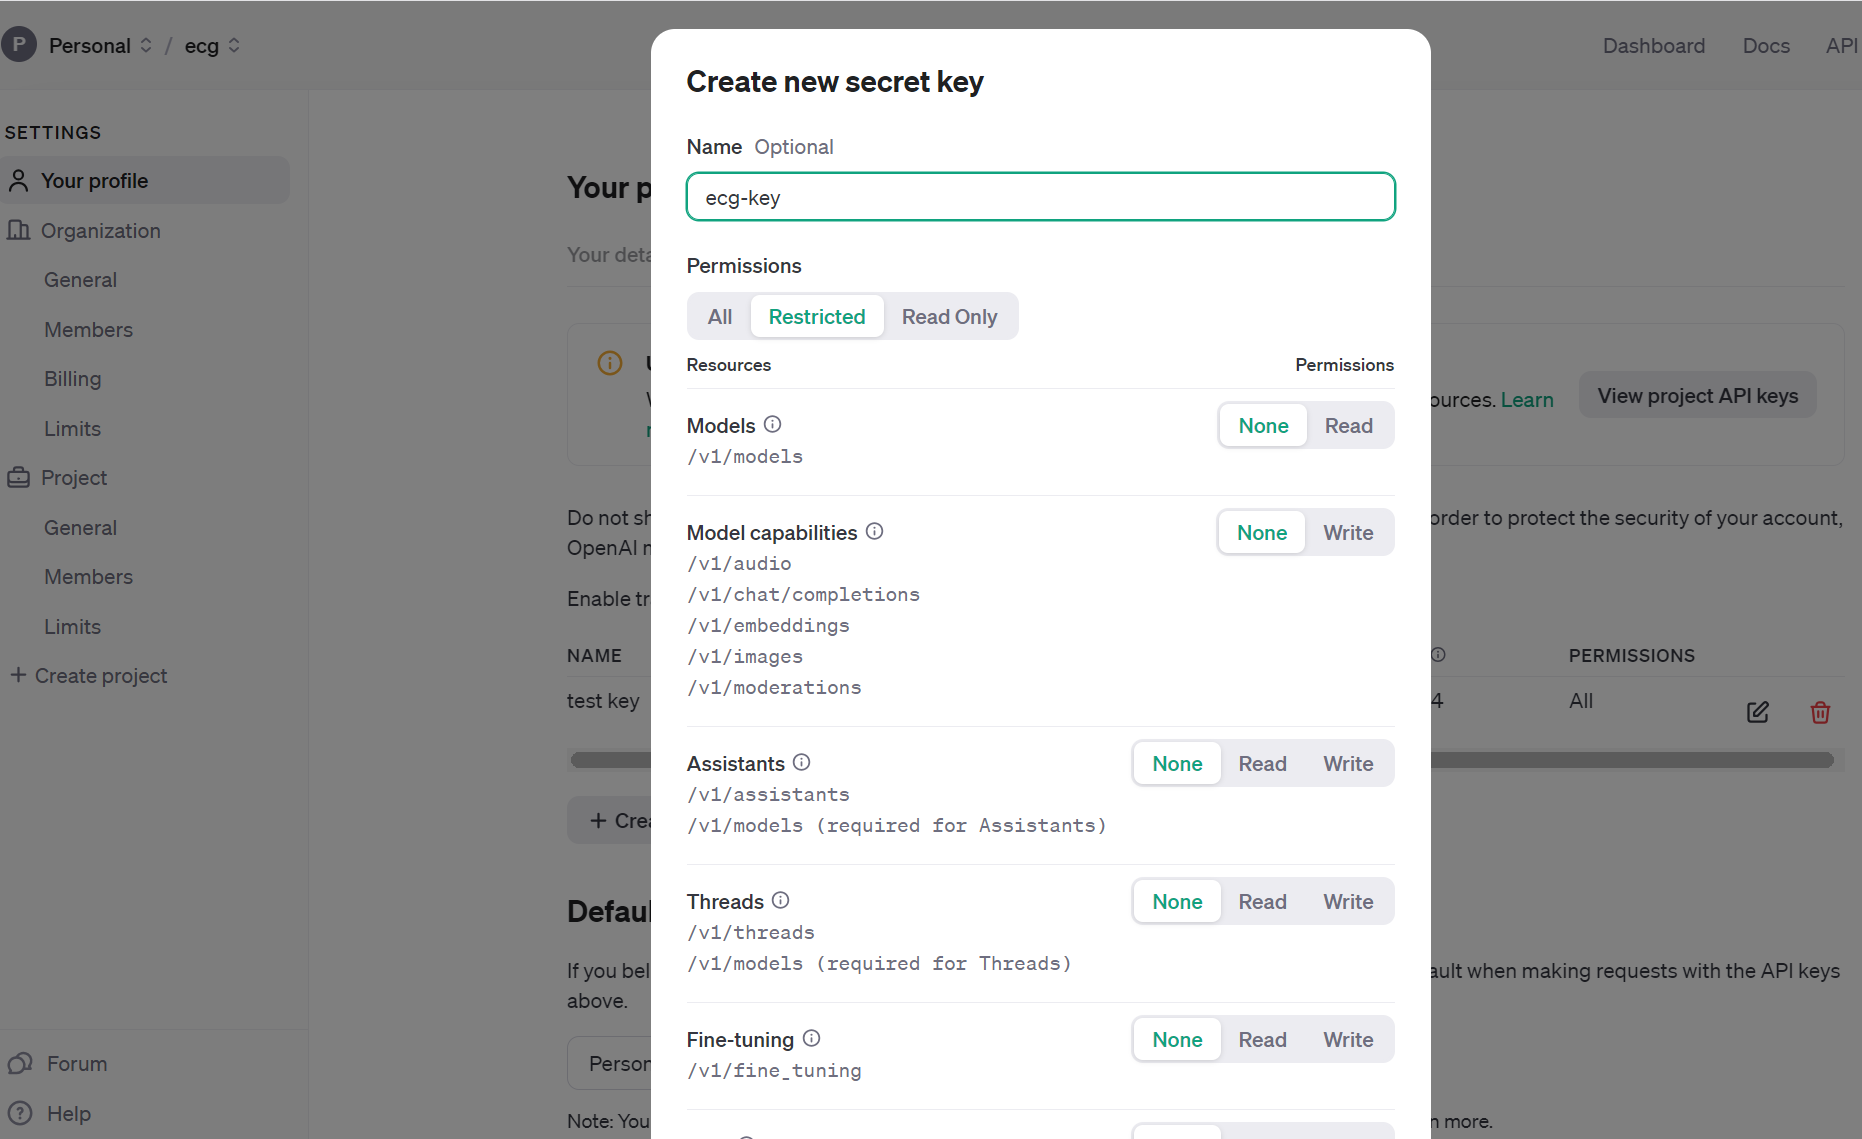
\includegraphics[scale=0.4]{Images/server/ai/private-key.png}
  \caption[Tạo key bảo mật cho API]{\bfseries \fontsize{12pt}{0pt}
  \selectfont Tạo key bảo mật cho API}
  \label{create-ai-project} %đặt tên cho ảnh
\end{figure}

Cung cấp dữ liệu ban đầu dưới dạng file .csv. Thông tin bao gồm giới thiệu chi tiết về các thành phần, cách sử dụng, người dùng của hệ thống.

\begin{figure}[H]
  \centering
  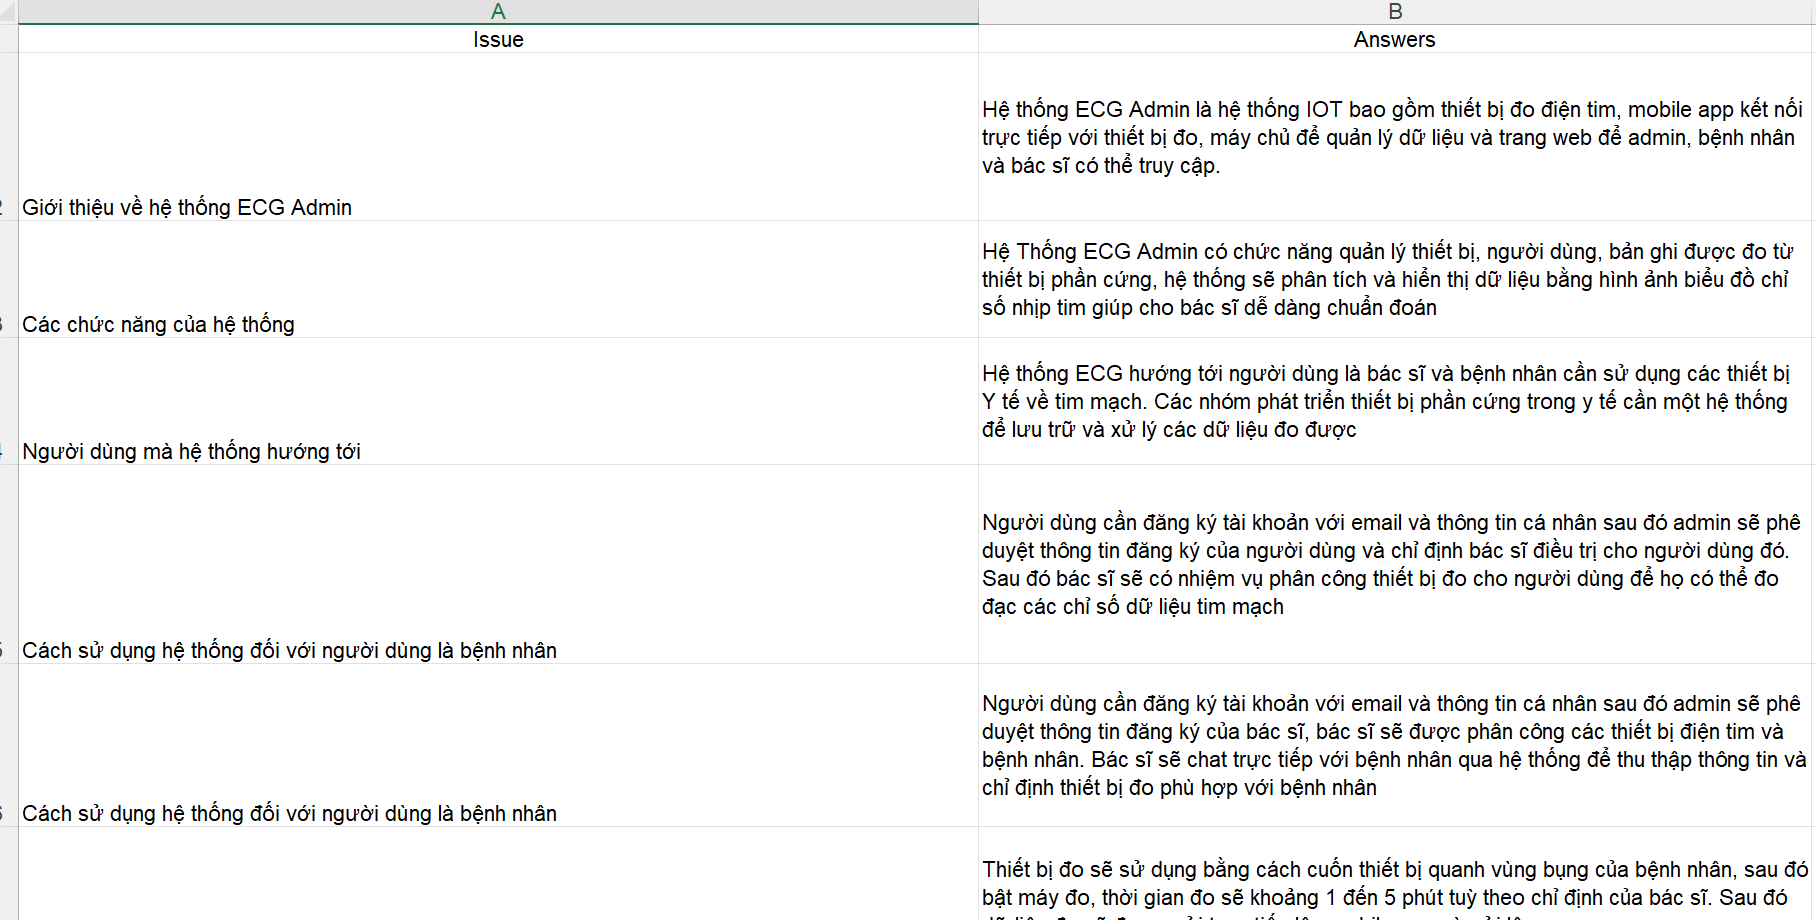
\includegraphics[scale=0.4]{Images/server/ai/training-ai.png}
  \caption[Cung cấp dữ liệu cho AI]{\bfseries \fontsize{12pt}{0pt}
  \selectfont Cung cấp dữ liệu cho AI}
  \label{create-ai-project} %đặt tên cho ảnh
\end{figure}

Tiếp theo đó, kiểm tra việc học dữ liệu của AI bằng cách đặt câu hỏi liên quan đến các vấn đề nằm trong file dữ liệu ban đầu, để đánh giá mức độ tiếp thu của model và hiệu chỉnh dữ liệu.

\begin{figure}[H]
  \centering
  
\includegraphics[scale=0.5]{Images/server/ai/check-ai.png}
  \caption[Kiểm tra độ chính xác câu trả lời của ai]{\bfseries \fontsize{12pt}{0pt}
  \selectfont Kiểm tra độ chính xác câu trả lời của ai}
  \label{check-ai} %đặt tên cho ảnh
\end{figure}

Sau khi hoàn tất các bước ta đã có một trợ lý ảo, nhưng trợ lý ảo sẽ không thể tiếp nhận cùng lúc được nhiều người dùng cùng hỏi. Do đó chúng em đã chia đoạn chat của từng người dùng với ai thành một luồng riêng biệt. Để ai có thể hiểu và hỗ trợ riêng biệt cho mỗi người dùng. Dữ liệu chat của người dùng với ai sẽ được lưu trữ và tiếp tục huấn luyện cho ai để ai co thể duy trì cuộc hội thoại với họ 

\begin{figure}[H]
  \centering
  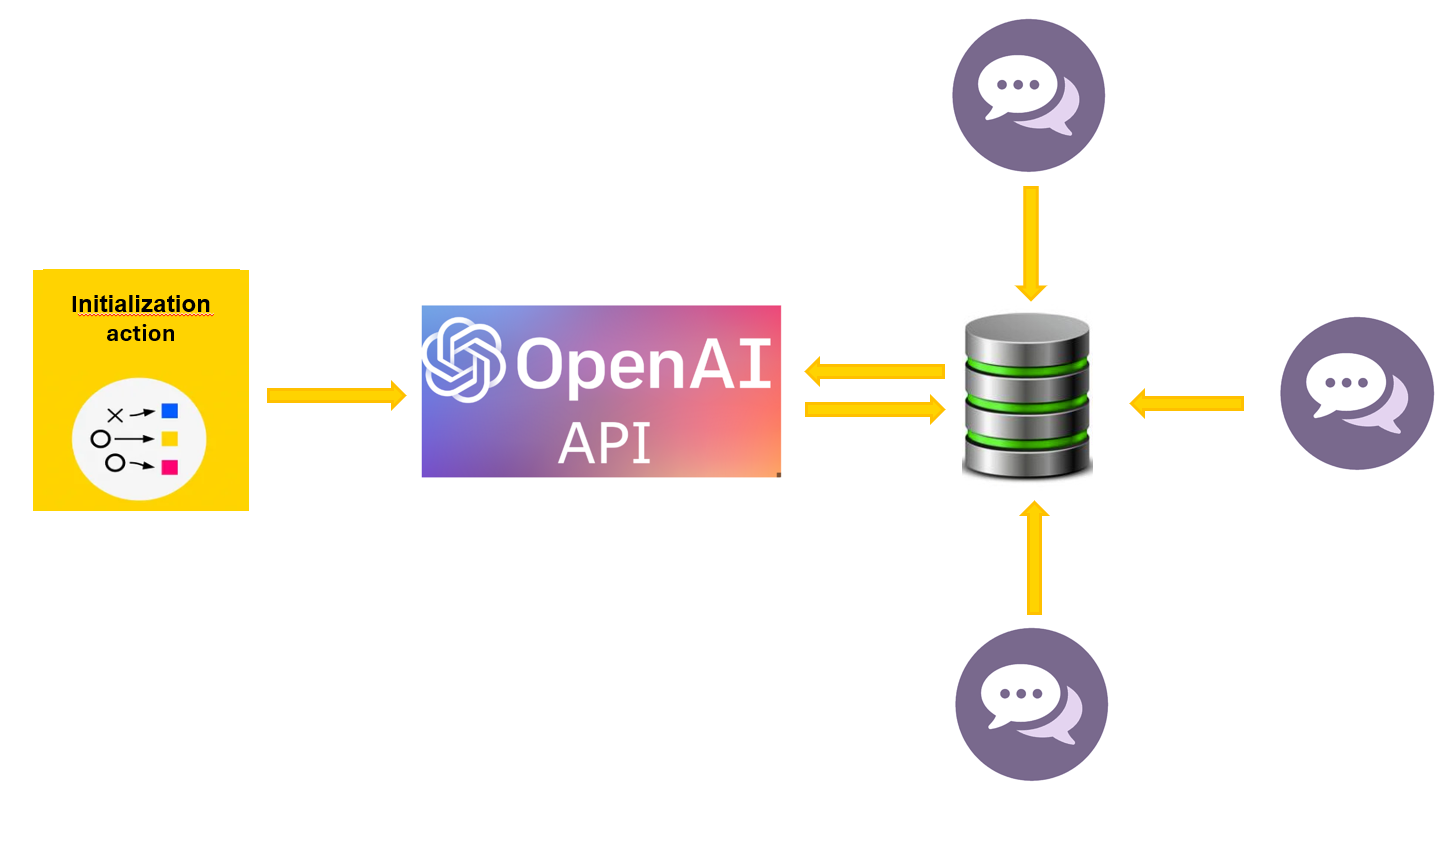
\includegraphics[scale=0.5]{Images/server/ai/tranning-ai-data.png}
  \caption[Phân luồng trò chuyện của từng người dùng]{\bfseries \fontsize{12pt}{0pt}
  \selectfont Phân luồng trò chuyện của từng người dùng}
  \label{thread-ai} %đặt tên cho ảnh
\end{figure}

Bây giờ môi cuộc trò chuyện giữa người dùng và AI sẽ diễn ra riêng biệt để AI có thể duy trì và trả lời chính xác.
\begin{figure}[H]
  \centering
  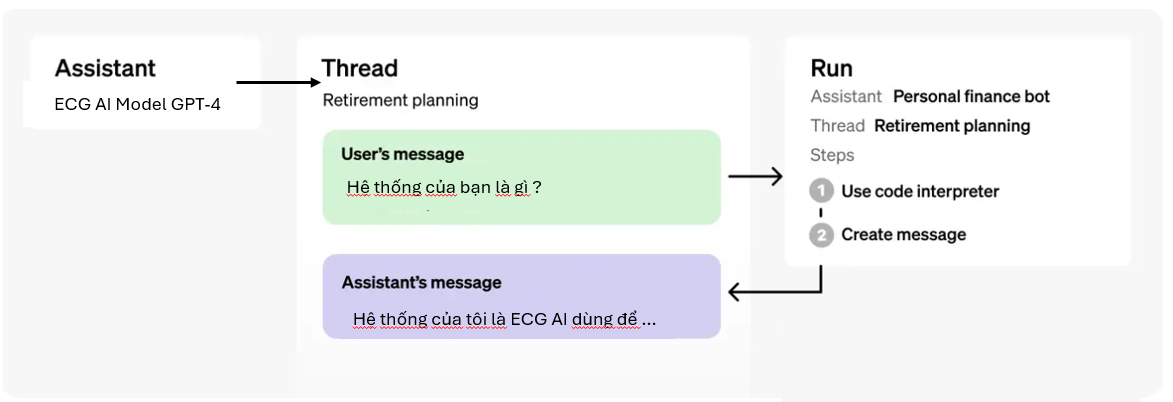
\includegraphics[scale=0.7]{Images/server/ai/thread-message.png}
  \caption[Mô hình hoạt động của từng cuộc hội thoại]{\bfseries \fontsize{12pt}{0pt}
  \selectfont Mô hình hoạt động của từng cuộc hội thoại}
  \label{check-ai} %đặt tên cho ảnh
\end{figure}

Sau khi hoàn tất chúng ta sẽ có được một trợ lý được tinh chỉnh dể phù hợp với hệ thống và cung cấp tư vấn chính xác cho từng người dùng với dữ liệu cá nhân của họ.

\subsection{Kiểm thử}

\subsubsection{Kiểm thử hoạt động của các API}


Môi trường: 

\begin{adjustwidth}{1.5em}{}
\begin{itemize}
  \item Base URL: http://103.200.20.59/ hoặc http://localhost:3000/
\end{itemize}
\end{adjustwidth}

Công cụ: Postman - Để xây dựng và thực hiện các yêu cầu API.

\paragraph{API liên quan đến việc xác thực người dùng}
\mbox{}

Tham khảo bảng \ref{table_api_auth} để xem thông tin của các api liên quan


\begin{enumerate}[a)]
  \item URL: POST api/auth/register
  
  \break
  \begin{xltabular}{\textwidth}{
    | >{\raggedright\arraybackslash}p{1cm}
    | >{\raggedright\arraybackslash}p{2.5cm}
    | >{\raggedright\arraybackslash}X
    | >{\raggedright\arraybackslash}X
    | >{\raggedright\arraybackslash}p{1cm}|
    }
    \caption{\bfseries \fontsize{12pt}{0pt}\selectfont Bảng kiểm thử API đăng ký tài khoản}
    % \label{table_api_news}
    \\
    \hline
    \bfseries Test case    &\bfseries Điều kiện   &\bfseries Đầu vào 
    &\bfseries Đầu ra mong muốn &\bfseries Kết quả\\ \hline
  
  
    TC-1
    & Người dùng chưa có tài khoản trên hệ thống
    & Thông tin đăng ký tài khoản

    \{

    "username": "Nguyen Van A",

    "password": "123456789",

    "email": "test@gmail.com",

    "birth": "",

    "gender": 1,

    "phone\_number": "0123344562",

    "role": 0

   \}
  
    & 
  
    Status code: 200 OK
  
      Response content:
  
      \{
  
    "status": "success",
  
    "message": "Your account is pending."
  
    \}
    
    & OK
  
    \\ \hline
  
    TC-2
    & Người dùng đã có tài khoản trên hệ thống
    & Thông tin đăng ký tài khoản

    \{

    "username": "Nguyen Van A",

    "password": "123456789",

    "email": "test@gmail.com",

    "birth": "",

    "gender": 1,

    "phone\_number": "0123344562",

    "role": 0

   \}
  
    & 
  
    Status code: 400 Bad Request
  
      Response content:
  
      \{
  
    "status": "error",
  
    "message": "Email has already been in use"
  
    \}
    
    & OK
  
    \\ \hline
    
  
    \end{xltabular}


  \item URL: POST api/auth/login
  

  \begin{xltabular}{\textwidth}{
    | >{\raggedright\arraybackslash}p{1cm}
    | >{\raggedright\arraybackslash}p{2.5cm}
    | >{\raggedright\arraybackslash}X
    | >{\raggedright\arraybackslash}X
    | >{\raggedright\arraybackslash}p{1cm}|
    }
    \caption{\bfseries \fontsize{12pt}{0pt}\selectfont Bảng kiểm thử API đăng nhập}
    % \label{table_api_news}
    \\
    \hline
    \bfseries Test case    &\bfseries Điều kiện   &\bfseries Đầu vào 
    &\bfseries Đầu ra mong muốn &\bfseries Kết quả\\ \hline
  
  
    TC-1
    & Thông tin tài khoản và mật khẩu hợp lệ
    & Thông tin đăng nhập

    \{

    "email": email người dùng,
    "password": mật khẩu người dùng

   \}
  
    & 
  
    Status code: 200 OK
  
      Response content:
  
      \{
  
    "status": "success",
  
    data: Thông tin user sau khi đăng ký thành công
  
    \}
    
    & OK
  
    \\ \hline
  
    TC-2
    & Thông tin tài khoản và mật khẩu không hợp lệ
    & Thông tin đăng nhập

    \{

    "email": email người dùng,
    "password": mật khẩu người dùng

   \}
  
   &
  
    Status code: 401 Unauthorized
  
      Response content:
  
      \{
  
    "status": "error",
  
    "message": "Invalid email or password"
  
    \}
    
    & OK
  
    \\ \hline

  
    \end{xltabular}



  \item URL: POST api/auth/logout
  

  \begin{xltabular}{\textwidth}{
    | >{\raggedright\arraybackslash}p{1cm}
    | >{\raggedright\arraybackslash}p{2.5cm}
    | >{\raggedright\arraybackslash}X
    | >{\raggedright\arraybackslash}X
    | >{\raggedright\arraybackslash}p{1cm}|
    }
    \caption{\bfseries \fontsize{12pt}{0pt}\selectfont Bảng kiểm thử API đăng xuất}
    % \label{table_api_news}
    \\
    \hline
    \bfseries Test case    &\bfseries Điều kiện   &\bfseries Đầu vào 
    &\bfseries Đầu ra mong muốn &\bfseries Kết quả\\ \hline
  
  
    TC-1
    & User đã đăng nhập vào hệ thống
    & JWT Token tồn tại
  
    & 
  
    Status code: 200 OK
  
      Response content:
  
      \{
  
    "status": "success",
  
    "message": "Logged out successfully"
  
    \}
    
    & OK
  
    \\ \hline
  
    TC-2
    & User chưa đăng nhập vào hệ thống
    & JWT Token không tồn tại
  
   &
  
    Status code: 401 Unauthorized
  
      Response content:
  
      \{
  
    "status": "error",
  
    "message": "No token found"
  
    \}
    
    & OK
  
    \\ \hline

  
    \end{xltabular}



  \item URL: POST api/auth/reset-password
  


  \begin{xltabular}{\textwidth}{
    | >{\raggedright\arraybackslash}p{1cm}
    | >{\raggedright\arraybackslash}p{2.5cm}
    | >{\raggedright\arraybackslash}X
    | >{\raggedright\arraybackslash}X
    | >{\raggedright\arraybackslash}p{1cm}|
    }
    \caption{\bfseries \fontsize{12pt}{0pt}\selectfont Bảng kiểm thử API gửi token đặt lại mật khẩu}
    % \label{table_api_news}
    \\
    \hline
    \bfseries Test case    &\bfseries Điều kiện   &\bfseries Đầu vào 
    &\bfseries Đầu ra mong muốn &\bfseries Kết quả\\ \hline
  
  
    TC-1
    & Người dùng đã đăng ký tài khoản
    & Email người dùng

    \{

    "email": email người dùng

    \}
    & 
  
    Status code: 200 OK
  
      Response content:
  
      \{
  
    "status": "success",
  
    "message": "Reset token sent to email"

    "resetToken": token
  
    \}
    
    & OK
  
    \\ \hline
  
    TC-2
    & Người dùng chưa đăng ký tài khoản
    & Email người dùng

    \{

    "email": email người dùng

    \}
   &
  
    Status code: 404 Not Found
  
      Response content:
  
      \{
  
    "status": "error",
  
    "message": "User not found"
  
    \}
    
    & OK
  
    \\ \hline

  
    \end{xltabular}



  \item URL: POST api/auth/reset-password/reset 
  


  \begin{xltabular}{\textwidth}{
    | >{\raggedright\arraybackslash}p{1cm}
    | >{\raggedright\arraybackslash}p{2.5cm}
    | >{\raggedright\arraybackslash}X
    | >{\raggedright\arraybackslash}X
    | >{\raggedright\arraybackslash}p{1cm}|
    }
    \caption{\bfseries \fontsize{12pt}{0pt}\selectfont Bảng kiểm thử API đặt lại mật khẩu}
    % \label{table_api_news}
    \\
    \hline
    \bfseries Test case    &\bfseries Điều kiện   &\bfseries Đầu vào 
    &\bfseries Đầu ra mong muốn &\bfseries Kết quả\\ \hline
  
  
    TC-1
    & User đã đăng ký tài khoản, reset token và mật khẩu hợp lệ
    & Thông tin reset mật khẩu

    \{

      "resetToken": "816e8d",

      "password": "123456",

      "email": "test@gmail.com"

  \}
  
    & 
  
    Status code: 200 OK
  
      Response content:
  
      \{
  
    "status": "success",
  
    "message": "Password reset successful"
  
    \}
    
    & OK
  
    \\ \hline
  
    TC-2
    & Reset token không hợp lệ
    & Thông tin reset mật khẩu

    \{

      "resetToken": "816e8d",

      "password": "123456",

      "email": "test@gmail.com"

  \}
   &
  
    Status code: 400 Bad Request
  
      Response content:
  
      \{
  
    "status": "error",
  
    "msg": "Invalid reset token"
  
    \}
    
    & OK
  
    \\ \hline

    TC-3
    & Reset token hết hạn
    & Thông tin reset mật khẩu

    \{

      "resetToken": "816e8d",

      "password": "123456",

      "email": "test@gmail.com"

  \}
   &
  
    Status code: 400 Bad Request
  
      Response content:
  
      \{
  
    "status": "error",
  
    "message": "Reset token has expired"
  
    \}
    
    & OK
  
    \\ \hline
    \end{xltabular}



\end{enumerate}

\paragraph{API liên quan đến việc xét duyệt đăng ký tài khoản}
\mbox{}

Tham khảo bảng \ref{table_api_register} để xem thông tin của các api liên quan



\begin{enumerate}[a)]
  \item URL: GET api/register/list
  
\break

  \begin{xltabular}{\textwidth}{
    | >{\raggedright\arraybackslash}p{1cm}
    | >{\raggedright\arraybackslash}p{2.5cm}
    | >{\raggedright\arraybackslash}p{3.5cm}
    | >{\raggedright\arraybackslash}X
    | >{\raggedright\arraybackslash}p{1cm}|
    }
    \caption{\bfseries \fontsize{12pt}{0pt}\selectfont Bảng kiểm thử API đăng ký tài khoản}
    % \label{table_api_news}
    \\
    \hline
    \bfseries Test case    &\bfseries Điều kiện   &\bfseries Đầu vào 
    &\bfseries Đầu ra mong muốn &\bfseries Kết quả\\ \hline
  
  
    TC-1
    & Người dùng là admin của hệ thống kèm theo token
    & Access token của người dùng trong Bearer Token
  
    & 
  
    Status code: 200 OK
  
      Response content:
  
      \{
  
    "status": "success",
  
    "data": Danh sách các tài khoản chờ phê duyệt
  
    \}
    
    & OK
  
    \\ \hline
  
    TC-2
    & Người dùng không phải là admin của hệ thống kèm theo token
    & Access token của người dùng trong Bearer Token
  
    & 
  
    Status code: 403 Forbidden
  
      Response content:
  
      \{
  
    "status": "error",
  
    "message": "You don't have permission to access"
  
    \}
    
    & OK
  
    \\ \hline
    TC-3
    & Yêu cầu không kèm theo token
    & NULL
  
    & 
  
    Status code: 401 Unauthorized  
  
      Response content:
  
      \{
  
    "status": "error",
  
    "message": "No token found"
  
    \}
    
    & OK
  
    \\ \hline
    
  
    \end{xltabular}


  \item URL: POST api/register/accepted
  

  \begin{xltabular}{\textwidth}{
    | >{\raggedright\arraybackslash}p{1cm}
    | >{\raggedright\arraybackslash}p{2.5cm}
    | >{\raggedright\arraybackslash}p{3.5cm}
    | >{\raggedright\arraybackslash}X
    | >{\raggedright\arraybackslash}p{1cm}|
    }
    \caption{\bfseries \fontsize{12pt}{0pt}\selectfont Bảng kiểm thử API chấp nhận tài khoản}
    % \label{table_api_news}
    \\
    \hline
    \bfseries Test case    &\bfseries Điều kiện   &\bfseries Đầu vào 
    &\bfseries Đầu ra mong muốn &\bfseries Kết quả\\ \hline
  
  
    TC-1
    & Tài khoản phê duyệt tồn tại trên hệ thống
    & ID tài khoản phê duyệt
  
    & 
  
    Status code: 200 OK
  
      Response content:
  
      \{
  
    "status": "success",
  
    "message": "Accept account successfully"
  
    \}
    & OK
  
    \\ \hline
  
    TC-2
    & Tài khoản phê duyệt không tồn tại trên hệ thống
    & ID tài khoản phê duyệt
  
   &
  
    Status code: 404 Not Found
  
      Response content:
  
      \{
  
    "status": "error",
  
    "message": "Register account not found"
  
    \}
    & OK
  
    \\ \hline

  
    \end{xltabular}



  \item URL: POST api/register/rejected
  

  \begin{xltabular}{\textwidth}{
    | >{\raggedright\arraybackslash}p{1cm}
    | >{\raggedright\arraybackslash}p{2.5cm}
    | >{\raggedright\arraybackslash}p{3.5cm}
    | >{\raggedright\arraybackslash}X
    | >{\raggedright\arraybackslash}p{1cm}|
    }
    \caption{\bfseries \fontsize{12pt}{0pt}\selectfont Bảng kiểm thử API từ chối phê duyệt tài khoản}
    % \label{table_api_news}
    \\
    \hline
    \bfseries Test case    &\bfseries Điều kiện   &\bfseries Đầu vào 
    &\bfseries Đầu ra mong muốn &\bfseries Kết quả\\ \hline
  
  
    TC-1
    & Tài khoản phê duyệt tồn tại trên hệ thống
    & ID tài khoản phê duyệt
  
    & 
  
    Status code: 200 OK
  
      Response content:
  
      \{
  
    "status": "success",
  
    "message": "Reject account successfully"
  
    \}
    
    & OK
  
    \\ \hline
  
    TC-2
    & Tài khoản phê duyệt tồn tại trên hệ thống
    & ID tài khoản phê duyệt
  
   &
  
    Status code: 404 Not Found
  
      Response content:
  
      \{
  
    "status": "error",
  
    "message": "Register account not found"
  
    \}
    
    & OK
  
    \\ \hline

  
    \end{xltabular}


\end{enumerate}


\paragraph{API liên quan đến thông tin người dùng}
\mbox{}

Tham khảo bảng \ref{table_api_user} để xem thông tin của các api liên quan

\begin{enumerate}[a)]
  \item URL: GET api/user
  

  \begin{xltabular}{\textwidth}{
    | >{\raggedright\arraybackslash}p{1cm}
    | >{\raggedright\arraybackslash}p{2.5cm}
    | >{\raggedright\arraybackslash}p{3.5cm}
    | >{\raggedright\arraybackslash}X
    | >{\raggedright\arraybackslash}p{1cm}|
    }
    \caption{\bfseries \fontsize{12pt}{0pt}\selectfont Bảng kiểm thử API lấy danh sách người dùng}
    % \label{table_api_news}
    \\
    \hline
    \bfseries Test case    &\bfseries Điều kiện   &\bfseries Đầu vào 
    &\bfseries Đầu ra mong muốn &\bfseries Kết quả\\ \hline
  
  
    TC-1
    & Người dùng là admin của hệ thống kèm theo token
    & Access token của người dùng trong Bearer Token
  
    & 
  
    Status code: 200 OK
  
      Response content:
  
      \{
  
    "status": "success",
  
    "data": Danh sách người dùng
  
    \}
    
    & OK
  
    \\ \hline
  
    TC-2
    & Người dùng không phải là admin của hệ thống kèm theo token
    & Access token của người dùng trong Bearer Token
  
    & 
  
    Status code: 403 Forbidden
  
      Response content:
  
      \{
  
    "status": "error",
  
    "message": "You don't have permission to access"
  
    \}
    
    & OK
  
    \\ \hline


    TC-3
    & Yêu cầu không kèm theo token
    & NULL
  
    & 
  
    Status code: 401 Unauthorized  
  
      Response content:
  
      \{
  
    "status": "error",
  
    "message": "No token found"
  
    \}
    
    & OK
  
    \\ \hline
    
  
    \end{xltabular}

  \item URL: GET api/user/id/{:userId}
    
  \begin{xltabular}{\textwidth}{
    | >{\raggedright\arraybackslash}p{1cm}
    | >{\raggedright\arraybackslash}p{2.5cm}
    | >{\raggedright\arraybackslash}p{2.5cm}
    | >{\raggedright\arraybackslash}X
    | >{\raggedright\arraybackslash}p{1cm}|
    }
    \caption{\bfseries \fontsize{12pt}{0pt}\selectfont Bảng kiểm thử API lấy thông tin của người dùng thông qua ID}
    % \label{table_api_news}
    \\
    \hline
    \bfseries Test case    &\bfseries Điều kiện   &\bfseries Đầu vào 
    &\bfseries Đầu ra mong muốn &\bfseries Kết quả\\ \hline
  
  
    TC-1
    & Người dùng tồn tại với ID tương ứng 
    & ID người dùng
  
    & 
  
    Status code: 200 OK
  
      Response content:
  
      \{
  
    "status": "success",
  
    data: Thông tin người dùng
  
    \}
    
    & OK
  
    \\ \hline
  
    TC-2
    & Người dùng không tồn tại với ID tương ứng
    & ID người dùng
  
    & 
  
    Status code: 404 Not Found
  
      Response content:
  
      \{
  
    "status": "error",
  
    "message": "User not found"
  
    \}
    
    & OK
  
    \\ \hline
    
  
    \end{xltabular}
  
  \item URL: GET api/user/{:role}
  
  \begin{xltabular}{\textwidth}{
    | >{\raggedright\arraybackslash}p{1cm}
    | >{\raggedright\arraybackslash}p{2.5cm}
    | >{\raggedright\arraybackslash}p{2cm}
    | >{\raggedright\arraybackslash}X
    | >{\raggedright\arraybackslash}p{1cm}|
    }
    \caption{\bfseries \fontsize{12pt}{0pt}\selectfont Bảng kiểm thử API lấy thông tin của người dùng thông qua chức vụ}
    % \label{table_api_news}
    \\
    \hline
    \bfseries Test case    &\bfseries Điều kiện   &\bfseries Đầu vào 
    &\bfseries Đầu ra mong muốn &\bfseries Kết quả\\ \hline
  
  
    TC-1
    & Role tồn tại trong CSDL 
    & Role
  
    & 
  
    Status code: 200 OK
  
      Response content:
  
      \{
  
    "status": "success",
  
    data: Danh sách người dùng ứng với role
  
    \}
    & OK
  
    \\ \hline
  
    TC-2
    & Role không tồn tại trong CSDL
    & Role
  
    & 
  
    Status code: 404 Not Found
  
      Response content:
  
      \{
  
    "status": "error",
  
    "message": "Role does not exist"
  
    \}
    & OK
  
    \\ \hline
    
  
    \end{xltabular}


  \item URL: POST api/user/update 
  
  \begin{xltabular}{\textwidth}{
    | >{\raggedright\arraybackslash}p{1cm}
    | >{\raggedright\arraybackslash}p{2cm}
    | >{\raggedright\arraybackslash}X
    | >{\raggedright\arraybackslash}X
    | >{\raggedright\arraybackslash}p{1cm}|
    }
    \caption{\bfseries \fontsize{12pt}{0pt}\selectfont Bảng kiểm thử API cập nhật thông tin người dùng}
  \\
  \hline
  \bfseries Test case    &\bfseries Điều kiện   &\bfseries Đầu vào 
  &\bfseries Đầu ra mong muốn &\bfseries Kết quả\\ \hline


  TC-1
  & Người dùng tồn tại với ID tương ứng
  & Thông tin cập nhật của người dùng
  \{

  "username": Họ và tên,

  "birth": Ngày sinh,

  "phone\_number": Số điện thoại,

  "gender": Giới tính,

  "status": Trạng thái

  \}
  & 

  Status code: 200 OK

    Response content:

    \{

  "status": "success",

  "data": Thông tin sau khi cập nhật của người dùng

  \}
  
  & OK

  \\ \hline

  TC-2
  & Người dùng không tồn tại với ID tương ứng
  & Thông tin cập nhật của người dùng

  \{

  "username": Họ và tên,

  "birth": Ngày sinh,

  "phone\_number": Số điện thoại,

  "gender": Giới tính,

  "status": Trạng thái

  \}
  & 

  Status code: 404 Not found

    Response content:

    \{

  "status": "error",

  "message": "User not found"

  \}
  
  & OK

  \\ \hline

  \end{xltabular}

  
  % TODO: Note new page
  \item URL: DELETE api/user/delete/{:userId}

  \begin{xltabular}{\textwidth}{
      | >{\raggedright\arraybackslash}p{1cm}
      | >{\raggedright\arraybackslash}p{2cm}
      | >{\raggedright\arraybackslash}p{2cm}
      | >{\raggedright\arraybackslash}X
      | >{\raggedright\arraybackslash}p{1cm}|
      }
      \caption{\bfseries \fontsize{12pt}{0pt}\selectfont Bảng kiểm thử API xóa thông tin người dùng}
    \\
    \hline
    \bfseries Test case    &\bfseries Điều kiện   &\bfseries Đầu vào 
    &\bfseries Đầu ra mong muốn &\bfseries Kết quả\\ \hline


    TC-1
    & Người dùng tồn tại với ID tương ứng
    & ID người dùng

    & 

    Status code: 200 OK

      Response content:

      \{

    "status": "success",

    "message": "Delete user successfully"

    \}
    
    & OK

    \\ \hline
  
    TC-2
    & Người dùng không tồn tại với ID tương ứng
    & ID người dùng

    & 

    Status code: 404 Not found

      Response content:

      \{

    "status": "error",

    "message": "User not found"

    \}
    
    & OK
    \\ \hline
  
    \end{xltabular}


\end{enumerate}


\paragraph{API liên quan đến thiết bị}
\mbox{}

Tham khảo bảng \ref{table_api_device} để xem thông tin của các api liên quan

\begin{enumerate}[a)]
  \item URL: GET api/device
    
    \begin{xltabular}{\textwidth}{
      | >{\raggedright\arraybackslash}p{1cm}
      | >{\raggedright\arraybackslash}p{2.5cm}
      | >{\raggedright\arraybackslash}p{2.5cm}
      | >{\raggedright\arraybackslash}X
      | >{\raggedright\arraybackslash}p{1cm}|
      }
      \caption{\bfseries \fontsize{12pt}{0pt}\selectfont Bảng kiểm thử API lấy danh sách thiết bị}
      % \label{table_api_news}
      \\
      \hline
      \bfseries Test case    &\bfseries Điều kiện   &\bfseries Đầu vào 
      &\bfseries Đầu ra mong muốn &\bfseries Kết quả\\ \hline
    
    
      TC-1
      & Người dùng đã đăng nhập vào hệ thống
      & Access token của người dùng trong Bearer Token
    
      & 
    
      Status code: 200 OK
    
        Response content:
    
        \{
    
      "status": "success",
    
      "data": Danh sách thiết bị
    
      \}
      & OK
    
      \\ \hline
    
      TC-2
      & Người dùng chưa đăng nhập vào hệ thống
      & Access token của người dùng trong Bearer Token
    
      & 
    
      Status code: 401 Unauthorized
    
        Response content:
    
        \{
    
      "status": "error",
    
      "message": "No token found"
    
      \}
      & OK
      \\ \hline

    
      \end{xltabular}
  

  \item URL: GET api/device/{:deviceId}
  
  \begin{xltabular}{\textwidth}{
    | >{\raggedright\arraybackslash}p{1cm}
    | >{\raggedright\arraybackslash}p{2.5cm}
    | >{\raggedright\arraybackslash}p{2.5cm}
    | >{\raggedright\arraybackslash}X
    | >{\raggedright\arraybackslash}p{1cm}|
    }
    \caption{\bfseries \fontsize{12pt}{0pt}\selectfont Bảng kiểm thử API lấy thông tin thiết bị theo ID}
    % \label{table_api_news}
    \\
    \hline
    \bfseries Test case    &\bfseries Điều kiện   &\bfseries Đầu vào 
    &\bfseries Đầu ra mong muốn &\bfseries Kết quả\\ \hline
  
  
    TC-1
    & Thiết bị tồn tại với ID tương ứng
    & ID thiết bị
    & 
  
    Status code: 200 OK
  
      Response content:
  
      \{
  
    "status": "success",

    data: Thông tin của thiết bị
  
    \}
    & OK
  
    \\ \hline
  
    TC-2
    & Thiết bị không tồn tại với ID tương ứng
    & ID thiết bị
   &
  
    Status code: 404 Not Found
  
      Response content:
  
      \{
  
    "status": "error",
  
    "message": "Device not found"
  
    \}
    & OK
  
    \\ \hline

  
    \end{xltabular}

  % //TODO: new page
  \item URL: POST api/device/add
  
  \begin{xltabular}{\textwidth}{
    | >{\raggedright\arraybackslash}p{1cm}
    | >{\raggedright\arraybackslash}p{2.5cm}
    | >{\raggedright\arraybackslash}X
    | >{\raggedright\arraybackslash}X
    | >{\raggedright\arraybackslash}p{1cm}|
    }
    \caption{\bfseries \fontsize{12pt}{0pt}\selectfont Bảng kiểm thử API thêm thiết bị}
    % \label{table_api_news}
    \\
    \hline
    \bfseries Test case    &\bfseries Điều kiện   &\bfseries Đầu vào 
    &\bfseries Đầu ra mong muốn &\bfseries Kết quả\\ \hline
  
  
    TC-1
    & Bệnh nhân và bác sĩ tồn tại với ID tương ứng
    & Thông tin thiết bị

    \{

    "device\_name": Tên thiết bị,

    "device\_type": Loại thiết bị,

    "user\_id": ID bệnh nhân,

    "doctor\_id": ID bác sĩ,

    "status": Trạng thái,

    "infomation": Thông tin thiết bị,

    "start\_date": Ngày bắt đầu sử dụng

   \}
    & 
  
    Status code: 200 OK
  
      Response content:
  
      \{
  
    "status": "success",
  
    data: Thông tin của thiết bị
  
    \}
    
    & OK
  
    \\ \hline
  
    TC-2
    & Bệnh nhân hoặc bác sĩ không tồn tại với ID tương ứng
    & Thông tin thiết bị

    \{

    "device\_name": Tên thiết bị,

    "device\_type": Loại thiết bị,

    "user\_id": ID bệnh nhân,

    "doctor\_id": ID bác sĩ,

    "status": Trạng thái,

    "infomation": Thông tin thiết bị,

    "start\_date": Ngày bắt đầu sử dụng

   \}
    & 
  
    Status code: 404 Not found
  
      Response content:
  
      \{
  
    "status": "error",
  
    "message": "User not found"
  
    \}
    
    & OK
  
    \\ \hline
    
  
    \end{xltabular}

  \item URL: POST api/device/update
  
  \begin{xltabular}{\textwidth}{
    | >{\raggedright\arraybackslash}p{1cm}
    | >{\raggedright\arraybackslash}p{2.5cm}
    | >{\raggedright\arraybackslash}X
    | >{\raggedright\arraybackslash}X
    | >{\raggedright\arraybackslash}p{1cm}|
    }
    \caption{\bfseries \fontsize{12pt}{0pt}\selectfont Bảng kiểm thử API cập nhật thông tin thiết bị}
    % \label{table_api_news}
    \\
    \hline
    \bfseries Test case    &\bfseries Điều kiện   &\bfseries Đầu vào 
    &\bfseries Đầu ra mong muốn &\bfseries Kết quả\\ \hline
  
  
    TC-1
    & Thiết bị tồn tại với ID tương ứng
    & Thông tin thiết bị

    \{

    "device\_name": Tên thiết bị,

    "device\_type": Loại thiết bị,

    "user\_id": ID bệnh nhân,

    "doctor\_id": ID bác sĩ,

    "status": Trạng thái,

    "infomation": Thông tin thiết bị,

    "start\_date": Ngày bắt đầu sử dụng

   \}
    & 
  
    Status code: 200 OK
  
      Response content:
  
      \{
  
    "status": "success",
  
    data: Thông tin sau khi cập nhật của thiết bị
  
    \}
    
    & OK
  
    \\ \hline
  
    TC-2
    & Thiết bị không tồn tại với ID tương ứng
    & Thông tin thiết bị

    \{

    "device\_name": Tên thiết bị,

    "device\_type": Loại thiết bị,

    "user\_id": ID bệnh nhân,

    "doctor\_id": ID bác sĩ,

    "status": Trạng thái,

    "infomation": Thông tin thiết bị,

    "start\_date": Ngày bắt đầu sử dụng

   \}
    & 
  
    Status code: 404 Not found
  
      Response content:
  
      \{
  
    "status": "error",
  
    "message": "Device not found"
  
    \}
    
    & OK
  
    \\ \hline

    TC-3
    & Bệnh nhân hoặc bác sĩ không tồn tại với ID tương ứng
    & Thông tin thiết bị

    \{

    "device\_name": Tên thiết bị,

    "device\_type": Loại thiết bị,

    "user\_id": ID bệnh nhân,

    "doctor\_id": ID bác sĩ,

    "status": Trạng thái,

    "infomation": Thông tin thiết bị,

    "start\_date": Ngày bắt đầu sử dụng

   \}
    & 
  
    Status code: 404 Not found
  
      Response content:
  
      \{
  
    "status": "error",
  
    "message": "User not found"
  
    \}
    
    & OK
  
    \\ \hline
  
    \end{xltabular}

  \item URL: DELETE api/device/delete/{:deviceId}
  
  \begin{xltabular}{\textwidth}{
    | >{\raggedright\arraybackslash}p{1cm}
    | >{\raggedright\arraybackslash}p{2.5cm}
    | >{\raggedright\arraybackslash}p{2.5cm}
    | >{\raggedright\arraybackslash}X
    | >{\raggedright\arraybackslash}p{1cm}|
    }
    \caption{\bfseries \fontsize{12pt}{0pt}\selectfont Bảng kiểm thử API xóa thiết bị}
    % \label{table_api_news}
    \\
    \hline
    \bfseries Test case    &\bfseries Điều kiện   &\bfseries Đầu vào 
    &\bfseries Đầu ra mong muốn &\bfseries Kết quả\\ \hline
  
  
    TC-1
    & Thiết bị tồn tại với ID tương ứng
    & ID thiết bị

    & 
  
    Status code: 200 OK
  
      Response content:
  
      \{
  
    "status": "success",
  
    "message": "Delete device successful"
  
    \}
    
    & OK
  
    \\ \hline
  
    TC-2
    & Thiết bị không tồn tại với ID tương ứng
    & ID thiết bị
  
    & 
  
    Status code: 404 Not found
  
      Response content:
  
      \{
  
    "status": "error",
  
    "message": "Device not found"
  
    \}
    
    & OK
  
    \\ \hline
    
  
    \end{xltabular}


\end{enumerate}



\paragraph{API liên quan đến bản ghi ECG}
\mbox{}

Tham khảo bảng \ref{table_api_ecg} để xem thông tin của các api liên quan

\begin{enumerate}[a)]
  \item URL: GET api/record
    
  \begin{xltabular}{\textwidth}{
    | >{\raggedright\arraybackslash}p{1cm}
    | >{\raggedright\arraybackslash}p{2.5cm}
    | >{\raggedright\arraybackslash}p{2.5cm}
    | >{\raggedright\arraybackslash}X
    | >{\raggedright\arraybackslash}p{1cm}|
    }
    \caption{\bfseries \fontsize{12pt}{0pt}\selectfont Bảng kiểm thử API lấy danh sách bản ghi}
    % \label{table_api_news}
    \\
    \hline
    \bfseries Test case    &\bfseries Điều kiện   &\bfseries Đầu vào 
    &\bfseries Đầu ra mong muốn &\bfseries Kết quả\\ \hline
  
  
    TC-1
    & Người dùng đăng nhập vào hệ thống
    & Access token của người dùng trong Bearer Token
  
    & 
  
    Status code: 200 OK
  
      Response content:
  
      \{
  
    "status": "success",
  
    data: Danh sách bản ghi 
  
    \}
    
    & OK
  
    \\ \hline
  
    TC-2
    & Người dùng chưa đăng nhập vào hệ thống
    & NULL
  
    & 
  
    Status code: 401 Unauthorized
  
      Response content:
  
      \{
  
    "status": "error",
  
    "message": "No token found"
  
    \}
    
    & OK
    \\ \hline

  
    \end{xltabular}

  
  \item URL: GET api/record/user/{:userId}
  
  \begin{xltabular}{\textwidth}{
    | >{\raggedright\arraybackslash}p{1cm}
    | >{\raggedright\arraybackslash}p{2.5cm}
    | >{\raggedright\arraybackslash}p{2.5cm}
    | >{\raggedright\arraybackslash}X
    | >{\raggedright\arraybackslash}p{1cm}|
    }
    \caption{\bfseries \fontsize{12pt}{0pt}\selectfont Bảng kiểm thử API lấy danh sách phiên đo ECG của bệnh nhân}
    % \label{table_api_news}
    \\
    \hline
    \bfseries Test case    &\bfseries Điều kiện   &\bfseries Đầu vào 
    &\bfseries Đầu ra mong muốn &\bfseries Kết quả\\ \hline
  
  
    TC-1
    & NULL
    & ID bệnh nhân

    & 
  
    Status code: 200 OK
  
      Response content:
  
      \{
  
    "status": "success",

    "data": Danh sách thông tin của tất cả phiên đo của bệnh nhân
  
    \}
    & OK
  
    \\ \hline
  
    TC-2
    & Lỗi đường truyền server
    & ID bệnh nhân

   &
  
    Status code: 500 Internal Server Error
  
      Response content:
  
      \{
  
    "status": "error",
  
    "message": "An error occurred while retrieving the records"
  
    \}
    & OK
  
    \\ \hline

  
    \end{xltabular}

  
  \item URL: GET api/record/doctor/{:doctorId}
  
  \begin{xltabular}{\textwidth}{
    | >{\raggedright\arraybackslash}p{1cm}
    | >{\raggedright\arraybackslash}p{2.5cm}
    | >{\raggedright\arraybackslash}p{2.5cm}
    | >{\raggedright\arraybackslash}X
    | >{\raggedright\arraybackslash}p{1cm}|
    }
    \caption{\bfseries \fontsize{12pt}{0pt}\selectfont Bảng kiểm thử API lấy danh sách phiên đo ECG mà bác sĩ phụ trách}
    % \label{table_api_news}
    \\
    \hline
    \bfseries Test case    &\bfseries Điều kiện   &\bfseries Đầu vào 
    &\bfseries Đầu ra mong muốn &\bfseries Kết quả\\ \hline
  
  
    TC-1
    & NULL
    & ID bác sĩ

    & 
  
    Status code: 200 OK
  
      Response content:
  
      \{
  
    "status": "success",

    "data": Danh sách thông tin của tất cả phiên đo mà bác sĩ phụ trách
  
    \}
    & OK
    \\ \hline
  
    TC-2
    & Lỗi đường truyền server
    & ID bác sĩ

   &
  
    Status code: 500 Internal Server Error
  
      Response content:
  
      \{
  
    "status": "error",
  
    "message": "An error occurred while retrieving the records"
  
    \}
    & OK
  
    \\ \hline

  
    \end{xltabular}

  \item URL: GET api/record/id/{:recordId}
  
  \begin{xltabular}{\textwidth}{
    | >{\raggedright\arraybackslash}p{1cm}
    | >{\raggedright\arraybackslash}p{2.5cm}
    | >{\raggedright\arraybackslash}p{2.5cm}
    | >{\raggedright\arraybackslash}X
    | >{\raggedright\arraybackslash}p{1cm}|
    }
    \caption{\bfseries \fontsize{12pt}{0pt}\selectfont Bảng kiểm thử API lấy thông tin một phiên đo ECG}
    % \label{table_api_news}
    \\
    \hline
    \bfseries Test case    &\bfseries Điều kiện   &\bfseries Đầu vào 
    &\bfseries Đầu ra mong muốn &\bfseries Kết quả\\ \hline
  
  
    TC-1
    & Phiên đo tồn tại với ID tương ứng
    & ID phiên đo 

    & 
  
    Status code: 200 OK
  
      Response content:
  
      \{
  
    "status": "success",

    data: Thông tin phiên đo ECG
  
    \}
    & OK
  
    \\ \hline
  
    TC-2
    & Phiên đo không tồn tại với ID tương ứng
    & ID phiên đo 

   &
  
    Status code: 404 Not Found
  
      Response content:
  
      \{
  
    "status": "error",
  
    "message": "Record not found"
  
    \}
    & OK
  
    \\ \hline

  
    \end{xltabular}


  \item URL: GET api/record/getData/{:recordId}
  

  \begin{xltabular}{\textwidth}{
    | >{\raggedright\arraybackslash}p{1cm}
    | >{\raggedright\arraybackslash}p{2.5cm}
    | >{\raggedright\arraybackslash}p{2.5cm}
    | >{\raggedright\arraybackslash}X
    | >{\raggedright\arraybackslash}p{1cm}|
    }
    \caption{\bfseries \fontsize{12pt}{0pt}\selectfont Bảng kiểm thử API lấy dữ liệu bản ghi một phiên đo ECG}
    % \label{table_api_news}
    \\
    \hline
    \bfseries Test case    &\bfseries Điều kiện   &\bfseries Đầu vào 
    &\bfseries Đầu ra mong muốn &\bfseries Kết quả\\ \hline
  
  
    TC-1
    & Phiên đo tồn tại với ID tương ứng
    & ID phiên đo 

    & 
  
    Status code: 200 OK
  
      Response content:
  
      \{
  
    "status": "success",

    data: Dữ liệu bản ghi phiên đo ECG
  
    \}
    
    & OK
  
    \\ \hline
  
    TC-2
    & Phiên đo không tồn tại với ID tương ứng
    & ID phiên đo 

   &
  
    Status code: 404 Not Found
  
      Response content:
  
      \{
  
    "status": "error",
  
    "message": "Record not found"
  
    \}
    & OK
  
    \\ \hline
    TC-3
    & Lỗi đường truyền server
    & ID phiên đo

   &
  
    Status code: 500 Internal Server Error
  
      Response content:
  
      \{
  
    "status": "error",
  
    "message": "An error occurred while retrieving the records"
  
    \}
    & OK
  
    \\ \hline

  
    \end{xltabular}  

  \item URL: GET api/record/download/{:recordId} 
  

  \begin{xltabular}{\textwidth}{
    | >{\raggedright\arraybackslash}p{1cm}
    | >{\raggedright\arraybackslash}p{2.5cm}
    | >{\raggedright\arraybackslash}p{2.5cm}
    | >{\raggedright\arraybackslash}X
    | >{\raggedright\arraybackslash}p{1cm}|
    }
    \caption{\bfseries \fontsize{12pt}{0pt}\selectfont Bảng kiểm thử API tải dữ liệu đo ECG}
    % \label{table_api_news}
    \\
    \hline
    \bfseries Test case    &\bfseries Điều kiện   &\bfseries Đầu vào 
    &\bfseries Đầu ra mong muốn &\bfseries Kết quả\\ \hline
  
  
    TC-1
    & Bản ghi tồn tại với ID phiên đo tương ứng
    & ID phiên đo

    & 
  
    Status code: 200 OK
  
      Response content:
  
      \{
  
    "status": "success",

    data: File bản ghi dữ liệu ECG
  
    \}
    & OK
  
    \\ \hline
  
    TC-2
    & Phiên đo không tồn tại với ID tương ứng
    & ID phiên đo 

   &
  
    Status code: 404 Not Found
  
      Response content:
  
      \{
  
    "status": "error",
  
    "message": "Record not found"
    \}
    
    & OK
  
    \\ \hline
    TC-3
    & Lỗi đường truyền server
    & ID phiên đo

   &
  
    Status code: 500 Internal Server Error
  
      Response content:
  
      \{
  
    "status": "error",
  
    "message": "An error occurred while downloading the record file"
  
    \}
    & OK
  
    \\ \hline

  
    \end{xltabular}

  
  \item URL: POST api/record/update
  

  \begin{xltabular}{\textwidth}{
    | >{\raggedright\arraybackslash}p{1cm}
    | >{\raggedright\arraybackslash}p{2cm}
    | >{\raggedright\arraybackslash}X
    | >{\raggedright\arraybackslash}X
    | >{\raggedright\arraybackslash}p{1cm}|
    }
    \caption{\bfseries \fontsize{12pt}{0pt}\selectfont Bảng kiểm thử API cập nhật thông tin phiên đo}
    % \label{table_api_news}
    \\
    \hline
    \bfseries Test case    &\bfseries Điều kiện   &\bfseries Đầu vào 
    &\bfseries Đầu ra mong muốn &\bfseries Kết quả\\ \hline
  
  
    TC-1
    & Phiên đo tồn tại với ID tương ứng
    & Thông tin phiên đo 
    \{

    "user\_id": ID bệnh nhân,

    "device\_id": ID thiết bị,

    "record\_type": Loại bản ghi,

    "start\_time": Thời gian bắt đầu,

    "end\_time": Thời gian kết thúc

   \}
    & 
  
    Status code: 200 OK
  
      Response content:
  
      \{
  
    "status": "success",

    "message": "Update record successful"
  
    \}
    
    & OK
  
    \\ \hline
  
    TC-2
    & Phiên đo không tồn tại với ID tương ứng
    & Thông tin phiên đo 
    \{

    "user\_id": ID bệnh nhân,

    "device\_id": ID thiết bị,

    "record\_type": Loại bản ghi,

    "start\_time": Thời gian bắt đầu,

    "end\_time": Thời gian kết thúc

   \} 

   &
  
    Status code: 404 Not Found
  
      Response content:
  
      \{
  
    "status": "error",
  
    "message": "Record not found"
  
    \}
    
    & OK
  
    \\ \hline
    TC-3
    & Thông tin người dùng hoặc thiết bị không tồn tại với ID tương ứng
    & Thông tin phiên đo 
    \{

    "user\_id": ID bệnh nhân,

    "device\_id": ID thiết bị,

    "record\_type": Loại bản ghi,

    "start\_time": Thời gian bắt đầu,

    "end\_time": Thời gian kết thúc

   \} 
   &
  
    Status code: 404 Not Found
  
      Response content:
  
      \{
  
    "status": "error",
  
    "message": "Update info error"
  
    \}
    & OK
  
    \\ \hline
    
  
    \end{xltabular}

  \item URL: DELETE api/record/delete/{:recordId}
  

  \begin{xltabular}{\textwidth}{
    | >{\raggedright\arraybackslash}p{1cm}
    | >{\raggedright\arraybackslash}p{2.5cm}
    | >{\raggedright\arraybackslash}p{2.5cm}
    | >{\raggedright\arraybackslash}X
    | >{\raggedright\arraybackslash}p{1cm}|
    }
    \caption{\bfseries \fontsize{12pt}{0pt}\selectfont Bảng kiểm thử API xóa thông tin một phiên đo ECG}
    % \label{table_api_news}
    \\
    \hline
    \bfseries Test case    &\bfseries Điều kiện   &\bfseries Đầu vào 
    &\bfseries Đầu ra mong muốn &\bfseries Kết quả\\ \hline
  
  
    TC-1
    & Phiên đo tồn tại với ID tương ứng
    & ID phiên đo 

    & 
  
    Status code: 200 OK
  
      Response content:
  
      \{
  
    "status": "success",

    "message": "Delete record successfull"
  
    \}
    & OK
  
    \\ \hline
  
    TC-2
    & Phiên đo không tồn tại với ID tương ứng
    & ID phiên đo 

   &
  
    Status code: 404 Not Found
  
      Response content:
  
      \{
  
    "status": "error",
  
    "message": "Record not found"
  
    \}
    & OK
  
    \\ \hline

  
    \end{xltabular}


\end{enumerate}


\paragraph{API liên quan liên quan đến việc phân công bác sĩ - bệnh nhân}
\mbox{}

Tham khảo bảng \ref{table_api_pda} để xem thông tin của các api liên quan

\begin{enumerate}[a)]
  \item URL: GET api/pda
    
  \begin{xltabular}{\textwidth}{
    | >{\raggedright\arraybackslash}p{1cm}
    | >{\raggedright\arraybackslash}p{2.5cm}
    | >{\raggedright\arraybackslash}p{2.5cm}
    | >{\raggedright\arraybackslash}X
    | >{\raggedright\arraybackslash}p{1cm}|
    }
    \caption{\bfseries \fontsize{12pt}{0pt}\selectfont Bảng kiểm thử API lấy danh sách phân công bác sĩ - bệnh nhân}
    % \label{table_api_news}
    \\
    \hline
    \bfseries Test case    &\bfseries Điều kiện   &\bfseries Đầu vào 
    &\bfseries Đầu ra mong muốn &\bfseries Kết quả\\ \hline
  
  
    TC-1
    & Người dùng truy cập với quyền admin
    & Access token của người dùng trong Bearer Token
  
    & 
  
    Status code: 200 OK
  
      Response content:
  
      \{
  
    "status": "success",
  
    data: Danh sách phân công bác sĩ bệnh nhân 
  
    \}
    & OK
  
    \\ \hline
  
    TC-2
    & Người dùng truy cập không phải với tư cách admin
    & NULL
  
    & 
  
    Status code: 403 Forbidden
  
    Response content:

    \{

  "status": "error",

  "message": "You don't have permission to access"

  \}
    & OK
    \\ \hline
    TC-3
    & Người dùng chưa đăng nhập
    & NULL
  
    & 
  
    Status code: 401 Unauthorized
  
      Response content:
  
      \{
  
    "status": "error",
  
    "message": "No token found"
  
    \}
    & OK
    \\ \hline

  
    \end{xltabular}


  \item URL: POST api/pda/create
  

  \begin{xltabular}{\textwidth}{
    | >{\raggedright\arraybackslash}p{1cm}
    | >{\raggedright\arraybackslash}p{2.5cm}
    | >{\raggedright\arraybackslash}X
    | >{\raggedright\arraybackslash}X
    | >{\raggedright\arraybackslash}p{1cm}|
    }
    \caption{\bfseries \fontsize{12pt}{0pt}\selectfont Bảng kiểm thử API tạo một phân công bác sĩ - bệnh nhân}
    % \label{table_api_news}
    \\
    \hline
    \bfseries Test case    &\bfseries Điều kiện   &\bfseries Đầu vào 
    &\bfseries Đầu ra mong muốn &\bfseries Kết quả\\ \hline
  
  
    TC-1
    & NULL
    & Thông tin phân công bác sĩ - bệnh nhân 
    \{

    "user\_id": ID bệnh nhân,

    "doctor\_id": ID bác sĩ,

    "start\_date": Ngày bắt đầu,

    "end\_date": Ngày kết thúc

   \}
    & 
  
    Status code: 200 OK
  
      Response content:
  
      \{
  
    "status": "success",
    data: Thông tin phân công
  
    \}
    
    & OK
  
    \\ \hline
  
    TC-2
    & Thông tin bệnh nhân hoặc bác sĩ không tồn tại với ID tương ứng
    & Thông tin phiên đo 
    \{

    "user\_id": ID bệnh nhân,

    "doctor\_id": ID bác sĩ,

    "start\_date": Ngày bắt đầu,

    "end\_date": Ngày kết thúc

   \} 
   &
  
    Status code: 404 Not Found
  
      Response content:
  
      \{
  
    "status": "error",
  
    "message": "User not found"
  
    \}
    
    & OK
  
    \\ \hline
    
  
    \end{xltabular}

  
  \item URL: POST api/pda/update
  

  \begin{xltabular}{\textwidth}{
    | >{\raggedright\arraybackslash}p{1cm}
    | >{\raggedright\arraybackslash}p{2cm}
    | >{\raggedright\arraybackslash}X
    | >{\raggedright\arraybackslash}X
    | >{\raggedright\arraybackslash}p{1cm}|
    }
    \caption{\bfseries \fontsize{12pt}{0pt}\selectfont Bảng kiểm thử API cập nhật thông tin phân công}
    % \label{table_api_news}
    \\
    \hline
    \bfseries Test case    &\bfseries Điều kiện   &\bfseries Đầu vào 
    &\bfseries Đầu ra mong muốn &\bfseries Kết quả\\ \hline
  
  
    TC-1
    & Phân công tồn tại với ID tương ứng
    & Thông tin phân công
    \{

    "user\_id": ID bệnh nhân,

    "doctor\_id": ID bác sĩ,

    "start\_date": Ngày bắt đầu,

    "end\_date": Ngày kết thúc

   \}
    & 
  
    Status code: 200 OK
  
      Response content:
  
      \{
  
    "status": "success",

    "message": "Update pda successful"
  
    \}
    & OK
  
    \\ \hline
  
    TC-2
    & Phân công không tồn tại với ID tương ứng
    & Thông tin phân công 
    \{

    "user\_id": ID bệnh nhân,

    "device\_id": ID thiết bị,

    "record\_type": Loại bản ghi,

    "start\_time": Thời gian bắt đầu,

    "end\_time": Thời gian kết thúc

   \} 
   &
  
    Status code: 404 Not Found
  
      Response content:
  
      \{
  
    "status": "error",
  
    "message": "PDA not found"
  
    \}
    & OK
  
    \\ \hline
    TC-3
    & Thông tin bác sĩ hoặc bệnh nhân không tồn tại với ID tương ứng
    & Thông tin phân công 
    \{

    "user\_id": ID bệnh nhân,

    "doctor\_id": ID bác sĩ,

    "start\_date": Ngày bắt đầu,

    "end\_date": Ngày kết thúc

   \} 

   &
  
    Status code: 404 Not Found
  
      Response content:
  
      \{
  
    "status": "error",
  
    "message": "User not found"
  
    \}
    & OK
  
    \\ \hline
    
  
    \end{xltabular}
  
  \item URL: DELETE api/pda/delete/{:pdaId}
  

  \begin{xltabular}{\textwidth}{
    | >{\raggedright\arraybackslash}p{1cm}
    | >{\raggedright\arraybackslash}p{2.5cm}
    | >{\raggedright\arraybackslash}p{2.5cm}
    | >{\raggedright\arraybackslash}X
    | >{\raggedright\arraybackslash}p{1cm}|
    }
    \caption{\bfseries \fontsize{12pt}{0pt}\selectfont Bảng kiểm thử API xóa thông tin phân công}
    % \label{table_api_news}
    \\
    \hline
    \bfseries Test case    &\bfseries Điều kiện   &\bfseries Đầu vào 
    &\bfseries Đầu ra mong muốn &\bfseries Kết quả\\ \hline
  
  
    TC-1
    & Phân công tồn tại với ID tương ứng
    & ID phân công 

    & 
  
    Status code: 200 OK
  
      Response content:
  
      \{
  
    "status": "success",

    "message": "Delete PDA successfull"
  
    \}
    & OK
  
    \\ \hline
  
    TC-2
    & Phân công không tồn tại với ID tương ứng
    & ID phân công 

   &
  
    Status code: 404 Not Found
  
      Response content:
  
      \{
  
    "status": "error",
  
    "message": "PDA not found"
  
    \}
    & OK
  
    \\ \hline

  
    \end{xltabular}

  \item URL: GET api/pda/patient/\{:doctorId\}
  
  \begin{xltabular}{\textwidth}{
    | >{\raggedright\arraybackslash}p{1cm}
    | >{\raggedright\arraybackslash}p{2.5cm}
    | >{\raggedright\arraybackslash}p{2.5cm}
    | >{\raggedright\arraybackslash}X
    | >{\raggedright\arraybackslash}p{1cm}|
    }
    \caption{\bfseries \fontsize{12pt}{0pt}\selectfont Bảng kiểm thử API lấy danh sách bệnh nhân mà bác sĩ đang quản lý theo ID bác sĩ}
    % \label{table_api_news}
    \\
    \hline
    \bfseries Test case    &\bfseries Điều kiện   &\bfseries Đầu vào 
    &\bfseries Đầu ra mong muốn &\bfseries Kết quả\\ \hline
  
  
    TC-1
    & NULL
    & ID bác sĩ

    & 
  
    Status code: 200 OK
  
      Response content:
  
      \{
  
    "status": "success",

    data: Thông tin của các bệnh nhân mà bác sỹ đang được phân công
  
    \}
    & OK
  
    \\ \hline
  
    TC-2
    & Bác sĩ không tồn tại với ID tương ứng
    & ID bác sĩ 

   &
  
    Status code: 404 Not Found
  
      Response content:
  
      \{
  
    "status": "error",
  
    "message": "Doctor not found"
  
    \}
    & OK
  
    \\ \hline

  
    \end{xltabular}

  \item URL: GET api/pda/doctor/\{:patientId\}

  \begin{xltabular}{\textwidth}{
    | >{\raggedright\arraybackslash}p{1cm}
    | >{\raggedright\arraybackslash}p{2.5cm}
    | >{\raggedright\arraybackslash}p{2.5cm}
    | >{\raggedright\arraybackslash}X
    | >{\raggedright\arraybackslash}p{1cm}|
    }
    \caption{\bfseries \fontsize{12pt}{0pt}\selectfont Bảng kiểm thử API lấy thông tin bác sĩ đang quản lý bệnh nhân theo ID bệnh nhân}
    % \label{table_api_news}
    \\
    \hline
    \bfseries Test case    &\bfseries Điều kiện   &\bfseries Đầu vào 
    &\bfseries Đầu ra mong muốn &\bfseries Kết quả\\ \hline
  
  
    TC-1
    & NULL
    & ID bệnh nhân

    & 
  
    Status code: 200 OK
  
      Response content:
  
      \{
  
    "status": "success",

    data: Thông tin của bác sỹ được phân công cho bệnh nhân
  
    \}
    & OK
  
    \\ \hline
  
    TC-2
    & Bệnh nhân không tồn tại với ID tương ứng
    & ID bệnh nhân 

   &
  
    Status code: 404 Not Found
  
      Response content:
  
      \{
  
    "status": "error",
  
    "message": "Patient not found"
  
    \}
    & OK
  
    \\ \hline

  
    \end{xltabular}

\end{enumerate}

\subsubsection{Kiểm thử ứng dụng web}

\begin{xltabular}{\textwidth}{
  | >{\raggedright\arraybackslash}p{2cm}
  | >{\raggedright\arraybackslash}X
  | >{\raggedright\arraybackslash}X
  | >{\raggedright\arraybackslash}p{1cm}|
  }
  \caption{\bfseries \fontsize{12pt}{0pt}\selectfont Bảng kiểm thử chức năng của website quản trị}
  % \label{table_api_news}
  \\
  \hline
  \bfseries Test case    &\bfseries Tái hiện 
  &\bfseries Kết quả mong muốn &\bfseries Đánh giá\\ \hline


  Kiểm tra chức năng đăng nhập
  & 1. Vào màn hình đăng nhập $\rightarrow$ Nhập thông tin tài khoản hoặc mật khẩu chưa có trên hệ thống
  $\rightarrow$ Nhấn nút đăng nhập

  % \\ &

  2. Vào màn hình đăng nhập $\rightarrow$ Nhập thông tin tài khoản hoặc mật khẩu hơp lệ
  $\rightarrow$ Nhấn nút đăng nhập 
  & 

1. Hiển thị thông báo sai email hoặc mật khẩu


2. Đăng nhập thành công vào hệ thống
  & OK

  \\ \hline

   
  Kiểm tra chức năng đăng ký
  & 

  1. Vào màn hình đăng ký $\rightarrow$ Nhập thông tin tài khoản đã có trên hệ thống
  $\rightarrow$ Nhấn nút đăng ký

  % \\ &

  2. Vào màn hình đăng ký $\rightarrow$ Nhập thông tin đăng ký hơp lệ
  $\rightarrow$ Nhấn nút đăng ký 
 
  & 


  1. Hiển thị thông báo email đã tồn tại trong hệ thông

  2. Hiển thị thông báo tài khoản đang chờ phê duyệt

  & OK

  \\ \hline
    Kiểm tra chức năng quản lý người dùng
  & 

1. Vào màn hình quản lý người dùng 

2. Xem thông tin người dùng

3. Sửa thông tin người dùng có sẵn  $\rightarrow$ Lưu thay đổi

4. Xóa một người dùng khỏi hệ thống
 
  & 

1. Hiển thị danh sách người dùng

2. Hiển thị thông tin cụ thể của người dùng

3. Cập nhật thông tin người dùng thành công

4. Xóa tài khoản người dùng khỏi hệ thống thành công

  & OK

  \\ \hline

  Kiểm tra chức năng xem danh sách bác sĩ
  & 

1. Vào màn hình danh sách bác sĩ phụ trách 

2. Xem thông tin cụ thể của bác sĩ
 
  & 

  1. Hiển thị danh sách bác sĩ

2. Hiển thị thông tin cụ thể bác sĩ


  & OK

  \\ \hline

  Kiểm tra chức năng xem danh sách bệnh nhân
  & 

1. Vào màn hình quản lý bệnh nhân 

2. Hiển thị thông tin cụ thể bệnh nhân

& 

1. Hiển thị danh sách bệnh nhân

2. Hiển thị thông tin cụ thể bệnh nhân

  & OK

  \\ \hline


  Kiểm tra chức năng quản lý thiết bị
  & 

1. Vào màn hình quản lý thiết bị 

2. Xem thông tin chi tiết thiết bị 

3. Thêm thiết bị mới với thông tin hợp lệ $\rightarrow$ Lưu thông tin

4. Sửa thông tin thiết bị có sẵn $\rightarrow$ Lưu thay đổi

5. Xóa một thiết bị khỏi hệ thống
 
  & 

1. Hiển thị danh sách thiết bị

2. Hiển thị thông tin chi tiết thiết bị

3. Thêm thiết bị thành công

4. Cập nhật thông tin thiết bị thành công

5. Xóa thiết bị khỏi hệ thống thành công

  & OK

  \\ \hline

  Kiểm tra chức năng quản lý phiên đo
  & 
 
  1. Vào màn hình quản lý phiên đo

  2. Sửa thông tin danh mục có sẵn $\rightarrow$ Lưu thay đổi

  3. Xem đồ thị một phiên đo

  4. Tải bản ghi phiên đo $\rightarrow$ Lưu tệp


  & 

1. Hiển thị danh sách phiên đo

2. Cập nhật thông tin phiên đo

3. Hiển thị đồ thị dữ liệu phiên đo

4. Tải file dữ liệu phiên đo thành công

  & OK

  \\ \hline

  Kiểm tra chức năng quản lý phân công bệnh nhân - bác sĩ
  & 
 
  1. Vào màn hình quản lý phân công 

  2. Phân công bệnh nhân cho bác sĩ $\rightarrow$ Lưu thông tin

  3. Sửa thông tin phân công có sẵn $\rightarrow$ Lưu thay đổi

  4. Hủy phân công bệnh nhân cho bác sĩ

  & 

1. Hiển thị danh sách phân công

2. Phân công thành công

3. Cập nhật thông tin phân công thành công

4. Hủy phân công thành công

  & OK

  \\ \hline

  Kiểm tra chức năng quản lý phê duyệt tài khoản
  & 
1. Vào màn hình quản lý phê duyệt tài khoản 

2. Phê duyệt/Từ chối tài khoản 
 
  & 

1. Hiển thị danh sách tài khoản phê duyệt

2. Phê duyệt/Từ chối tài khoản thành công


  & OK


  \\ \hline
  
  Kiểm tra chức năng quản lý thông tin cá nhân
  & 
1. Vào màn hình quản lý thông tin cá nhân 

2. Sửa thông tin cá nhân có sẵn $\rightarrow$ Lưu thông tin
 
  & 

1. Hiển thị thông tin tài khoản cá nhân

2. Cập nhật thông tin cá nhân thành công


  & OK


  \\ \hline
  Kiểm tra chức năng nhắn tin
  & 
1. Vào màn hình nhắn tin bệnh nhân/bác sĩ

2. Nhập và gửi tin nhắn 
 
  & 

1. Hiển thị danh sách các cuộc hội thoại

2. Hiển thị tin nhắn lên màn hình


  & OK


  \\ \hline
  Kiểm tra chức năng hỏi, nhận tư vấn từ trợ lý ảo
  & 
1. Vào màn hình nhắn tin với trợ lý ảo

2. Nhập và gửi tin nhắn 
 
  & 

1. Hiển thị màn hình nhắn tin với trợ lý ảo

2. Hiển thị tin nhắn lên màn hình và phản hồi từ trợ lý ảo


  & OK


  \\ \hline

  \end{xltabular}


\subsection{Kết luận chương}
  Trong Chương 4, chúng em đã trình bày phần triển khai hệ thống trên những nền tảng cụ thể, kèm với đó là việc thực hiện
  các kiểm thử với mục tiêu rõ ràng, việc kiểm thử đã giúp chúng em có cái nhìn toàn diện cũng như rất chi tiết về cách đánh giá 
  hệ thống trong môi trường phát triển và thực tế, đồng thời chúng em cũng rút ra được những thiết sót và kinh nghiệm
  để có hướng phát triển cho những chức năng còn thiếu sót trong hệ thống.
\newpage
